\documentclass[a4paper,13pt,2p]{report}

\usepackage{graphicx}
\usepackage[font=normalsize]{caption}
\usepackage{subcaption}
\usepackage{float}
\usepackage{wrapfig}
\usepackage{amssymb}
\usepackage{amsmath}
\usepackage{amstext}
\usepackage[linesnumbered,ruled]{algorithm2e}
\usepackage{multicol}
\usepackage{multirow}
\usepackage{textcomp}

\usepackage[bookmarks=false]{hyperref}
\hypersetup{colorlinks,
	linkcolor=blue,
	citecolor=blue,
	urlcolor=blue}
\usepackage{titlesec}
\setcounter{secnumdepth}{4}

%\usepackage{csquotes}
%\usepackage[style=verbose-ibid,backend=bibtex]{biblatex}
%\bibliography{reference}

\titleformat{\paragraph}
{\normalfont\normalsize\bfseries}{\theparagraph}{0.25em}{}

\graphicspath{ {./images/} }
\usepackage[X2,T1]{fontenc}

\usepackage[left=3.5cm,right=2.5cm,top=2cm,bottom=2cm]{geometry}
\usepackage{indentfirst}
\usepackage{color, colortbl}
\definecolor{Gray}{gray}{0.9}

\usepackage{graphicx}
\graphicspath{{./images/}}	% declare the path(s) where your graphic files are
\DeclareGraphicsExtensions{.pdf,.jpeg,.png} % and their extensions so you won't have to specify these with every instance of \includegraphics
%%%%%%%%%%%%%%%%%%%%%%%%%%%%%%%%%%%%%%%%%%%%%%%%%%%%%%%%%%%%%%%%%%%%%%%%%%%%%%%%%%%%%%%%%%%

\usepackage{graphicx}
\usepackage{verbatim}
\usepackage{latexsym}
\usepackage{mathchars}
\usepackage{setspace}
\usepackage{footnote}

\setlength{\parskip}{\medskipamount}  % a little space before a \par
\setlength{\parindent}{0pt}	      % don't indent first lines of paragraphs
%UHEAD.STY  If this is included after \documentstyle{report}, it adds
% an underlined heading style to the LaTeX report style.
% \pagestyle{uheadings} will put underlined headings at the top
% of each page. The right page headings are the Chapter titles and
% the left page titles are supplied by \def\lefthead{text}.

% Ted Shapin, Dec. 17, 1986

\makeatletter
\def\chapapp2{Chapter}

\def\appendix{\par
 \setcounter{chapter}{0}
 \setcounter{section}{0}
 \def\chapapp2{Appendix}
 \def\@chapapp{Appendix}
 \def\thechapter{\Alph{chapter}}}

\def\ps@uheadings{\let\@mkboth\markboth
% modifications
\def\@oddhead{\protect\underline{\protect\makebox[\textwidth][l]
		{\sl\rightmark\hfill\rm\thepage}}}
\def\@oddfoot{}
\def\@evenfoot{}
\def\@evenhead{\protect\underline{\protect\makebox[\textwidth][l]
		{\rm\thepage\hfill\sl\leftmark}}}
% end of modifications
\def\chaptermark##1{\markboth {\ifnum \c@secnumdepth >\m@ne
 \chapapp2\ \thechapter. \ \fi ##1}{}}%
\def\sectionmark##1{\markright {\ifnum \c@secnumdepth >\z@
   \thesection. \ \fi ##1}}}
\makeatother
%%From: marcel@cs.caltech.edu (Marcel van der Goot)
%%Newsgroups: comp.text.tex
%%Subject: illegal modification of boxit.sty
%%Date: 28 Feb 92 01:10:02 GMT
%%Organization: California Institute of Technology (CS dept)
%%Nntp-Posting-Host: andromeda.cs.caltech.edu
%%
%%
%%Quite some time ago I posted a file boxit.sty; maybe it made it
%%to some archives, although I don't recall submitting it. It defines
%%	\begin{boxit}
%%	...
%%	\end{boxit}
%%to draw a box around `...', where the `...' can contain other
%%environments (e.g., a verbatim environment). Unfortunately, it had
%%a problem: it did not work if you used it in paragraph mode, i.e., it
%%only worked if there was an empty line in front of \begin{boxit}.
%%Luckily, that is easily corrected.
%%
%%HOWEVER, apparently someone noticed the problem, tried to correct it,
%%and then distributed this modified version. That would be fine with me,
%%except that:
%%1. There was no note in the file about this modification, it only has my
%%   name in it.
%%2. The modification is wrong: now it only works if there is *no* empty
%%   line in front of \begin{boxit}. In my opinion this bug is worse than
%%   the original one.
%%
%%In particular, the author of this modification tried to force an empty
%%line by inserting a `\\' in the definition of \Beginboxit. If you have
%%a version of boxit.sty with a `\\', please delete it. If you have my
%%old version of boxit.sty, please also delete it. Below is an improved
%%version.
%%
%%Thanks to Joe Armstrong for drawing my attention to the bug and to the
%%illegal version.
%%
%%                                          Marcel van der Goot
%% .---------------------------------------------------------------
%% | Blauw de viooltjes,                    marcel@cs.caltech.edu
%% |    Rood zijn de rozen;
%% | Een rijm kan gezet
%% |    Met plaksel en dozen.
%% |


% boxit.sty
% version: 27 Feb 1992
%
% Defines a boxit environment, which draws lines around its contents.
% Usage:
%   \begin{boxit}
%	... (text you want to be boxed, can contain other environments)
%   \end{boxit}
%
% The width of the box is the width of the contents.
% The boxit* environment behaves the same, except that the box will be
% at least as wide as a normal paragraph.
%
% The reason for writing it this way (rather than with the \boxit#1 macro
% from the TeXbook), is that now you can box verbatim text, as in
%   \begin{boxit}
%   \begin{verbatim}
%   this better come out in boxed verbatim mode ...
%   \end{verbatim}
%   \end{boxit}
%
%						Marcel van der Goot
%						marcel@cs.caltech.edu
%

\def\Beginboxit
   {\par
    \vbox\bgroup
	   \hrule
	   \hbox\bgroup
		  \vrule \kern1.2pt %
		  \vbox\bgroup\kern1.2pt
   }

\def\Endboxit{%
			      \kern1.2pt
		       \egroup
		  \kern1.2pt\vrule
		\egroup
	   \hrule
	 \egroup
   }	

\newenvironment{boxit}{\Beginboxit}{\Endboxit}
\newenvironment{boxit*}{\Beginboxit\hbox to\hsize{}}{\Endboxit}
\pagestyle{empty}

\setlength{\parskip}{2ex plus 0.5ex minus 0.2ex}
\setlength{\parindent}{0pt}

\makeatletter  %to avoid error messages generated by "\@". Makes Latex treat "@" like a letter

\linespread{1.5}
\def\zzfl@error{Float(s) lost}
\def\submitdate#1{\gdef\@submitdate{#1}}
\def\maketitle{
  \begin{titlepage}{
    %\linespread{1.5}
    \Large HANOI UNIVERSITY OF SCIENCE AND TECHNOLOGY \\
    %\linebreak
    School of Information and Comunication Technology \\
    %\linebreak
    *****
    \rm
    \vskip 0.5in
    
\includegraphics[width=0.2 \textwidth]{images/hust} 
    \vskip 0.5in
    \Large \bf GRADUATION THESIS\par
    \Large \flushleft Topic:\par
    \Large \center \bf \@title \par
  }

  \vskip 0.3in
  \par
 % \begin{flushright}
  {\Large Author: \bf \@author} 
  \vskip 0.1in
  \Large Supervisor: \bf PhD. Binh Minh Nguyen
%	\end{flushright}
  \par
  \vskip 2in
  \par
  
  \@submitdate
  \vfil
  \end{titlepage}
}

\def\titlepage{
  \newpage
  \centering
  \linespread{1}
  \normalsize
  \vbox to \vsize\bgroup\vbox to 9in\bgroup
}
\def\endtitlepage{
  \par
  \kern 0pt
  \egroup
  \vss
  \egroup
  \cleardoublepage
}

\def\abstract{
  \begin{center}{
    \Large\bf Tóm tắt}
  \end{center}
  \small
  %\def\baselinestretch{1.5}
  \linespread{1.5}
  \normalsize
}
\def\endabstract{
  \par
}

\newenvironment{sameauthor}{
	\cleardoublepage
	\begin{center}{
			\large \bf PHỤ LỤC 1: GIẤY XÁC NHẬN ĐỒNG TÁC GIẢ}
	\end{center}
	\small
	\linespread{1.5}
	\normalsize
}{\cleardoublepage}
\def\endsameauthor{
	\par
}


\newenvironment{acknowledgements}{
  \cleardoublepage
  \begin{center}{
    \large \bf Lời cảm ơn}
  \end{center}
  \small
  \linespread{1.5}
  \normalsize
}{\cleardoublepage}
\def\endacknowledgements{
  \par
}

\newenvironment{dedication}{
  \cleardoublepage
  \begin{center}{
    \large \bf Lời cam đoan}
  \end{center}
  \small
  \linespread{1.5}
  \normalsize
}{\cleardoublepage}
\def\enddedication{
  \par
}

\def\preface{

    \pagestyle{plain}
    \doublespacing
}

\def\body{
    \cleardoublepage    
    \pagestyle{uheadings}
    \tableofcontents
    \pagestyle{plain}
    \cleardoublepage
    \pagestyle{uheadings}
    \listoftables
    \pagestyle{plain}
    \cleardoublepage
    \pagestyle{uheadings}
    \listoffigures
    \pagestyle{plain}
    \cleardoublepage
    \pagestyle{uheadings}
    
    \doublespacing
}

\pagenumbering{arabic}
\makeatother  %to avoid error messages generated by "\@". Makes Latex treat "@" like a letter

\newcommand{\ipc}{{\sf ipc}}

\newcommand{\Prob}{\bbbp}
\newcommand{\Real}{\bbbr}
\newcommand{\real}{\Real}
\newcommand{\Int}{\bbbz}
\newcommand{\Nat}{\bbbn}

\newcommand{\NN}{{\sf I\kern-0.14emN}}   % Natural numbers
\newcommand{\ZZ}{{\sf Z\kern-0.45emZ}}   % Integers
\newcommand{\QQQ}{{\sf C\kern-0.48emQ}}   % Rational numbers
\newcommand{\RR}{{\sf I\kern-0.14emR}}   % Real numbers
\newcommand{\KK}{{\cal K}}
\newcommand{\OO}{{\cal O}}
\newcommand{\AAA}{{\bf A}}
\newcommand{\HH}{{\bf H}}
\newcommand{\II}{{\bf I}}
\newcommand{\LL}{{\bf L}}
\newcommand{\PP}{{\bf P}}
\newcommand{\PPprime}{{\bf P'}}
\newcommand{\QQ}{{\bf Q}}
\newcommand{\UU}{{\bf U}}
\newcommand{\UUprime}{{\bf U'}}
\newcommand{\zzero}{{\bf 0}}
\newcommand{\ppi}{\mbox{\boldmath $\pi$}}
\newcommand{\aalph}{\mbox{\boldmath $\alpha$}}
\newcommand{\bb}{{\bf b}}
\newcommand{\ee}{{\bf e}}
\newcommand{\mmu}{\mbox{\boldmath $\mu$}}
\newcommand{\vv}{{\bf v}}
\newcommand{\xx}{{\bf x}}
\newcommand{\yy}{{\bf y}}
\newcommand{\zz}{{\bf z}}
\newcommand{\oomeg}{\mbox{\boldmath $\omega$}}
\newcommand{\res}{{\bf res}}
\newcommand{\cchi}{{\mbox{\raisebox{.4ex}{$\chi$}}}}
%\newcommand{\cchi}{{\cal X}}
%\newcommand{\cchi}{\mbox{\Large $\chi$}}

% Logical operators and symbols
\newcommand{\imply}{\Rightarrow}
\newcommand{\bimply}{\Leftrightarrow}
\newcommand{\union}{\cup}
\newcommand{\intersect}{\cap}
\newcommand{\boolor}{\vee}
\newcommand{\booland}{\wedge}
\newcommand{\boolimply}{\imply}
\newcommand{\boolbimply}{\bimply}
\newcommand{\boolnot}{\neg}
\newcommand{\boolsat}{\!\models}
\newcommand{\boolnsat}{\!\not\models}


\newcommand{\op}[1]{\mathrm{#1}}
\newcommand{\s}[1]{\ensuremath{\mathcal #1}}

% Properly styled differentiation and integration operators
\newcommand{\diff}[1]{\mathrm{\frac{d}{d\mathit{#1}}}}
\newcommand{\diffII}[1]{\mathrm{\frac{d^2}{d\mathit{#1}^2}}}
\newcommand{\intg}[4]{\int_{#3}^{#4} #1 \, \mathrm{d}#2}
\newcommand{\intgd}[4]{\int\!\!\!\!\int_{#4} #1 \, \mathrm{d}#2 \, \mathrm{d}#3}

% Large () brackets on different lines of an eqnarray environment
\newcommand{\Leftbrace}[1]{\left(\raisebox{0mm}[#1][#1]{}\right.}
\newcommand{\Rightbrace}[1]{\left.\raisebox{0mm}[#1][#1]{}\right)}

% Funky symobols for footnotes
\newcommand{\symbolfootnote}{\renewcommand{\thefootnote}{\fnsymbol{footnote}}}
% now add \symbolfootnote to the beginning of the document...

\newcommand{\normallinespacing}{\renewcommand{\baselinestretch}{1.5} \normalsize}
\newcommand{\mediumlinespacing}{\renewcommand{\baselinestretch}{1.2} \normalsize}
\newcommand{\narrowlinespacing}{\renewcommand{\baselinestretch}{1.0} \normalsize}
\newcommand{\bump}{\noalign{\vspace*{\doublerulesep}}}
\newcommand{\cell}{\multicolumn{1}{}{}}
\newcommand{\spann}{\mbox{span}}
\newcommand{\diagg}{\mbox{diag}}
\newcommand{\modd}{\mbox{mod}}
\newcommand{\minn}{\mbox{min}}
\newcommand{\andd}{\mbox{and}}
\newcommand{\forr}{\mbox{for}}
\newcommand{\EE}{\mbox{E}}

\newcommand{\deff}{\stackrel{\mathrm{def}}{=}}
\newcommand{\syncc}{~\stackrel{\textstyle \rhd\kern-0.57em\lhd}{\scriptstyle L}~}

\def\coop{\mbox{\large $\rhd\!\!\!\lhd$}}
\newcommand{\sync}[1]{\raisebox{-1.0ex}{$\;\stackrel{\coop}{\scriptscriptstyle
#1}\,$}}

\newtheorem{definition}{Definition}[chapter]
\newtheorem{theorem}{Theorem}[chapter]

\newcommand{\Figref}[1]{Figure~\ref{#1}}
\newcommand{\fig}[3]{
 \begin{figure}[!ht]
 \begin{center}
 \scalebox{#3}{\includegraphics{figs/#1.ps}}
 \vspace{-0.1in}
 \caption[ ]{\label{#1} #2}
 \end{center}
 \end{figure}
}

\newcommand{\figtwo}[8]{
 \begin{figure}
 \parbox[b]{#4 \textwidth}{
 \begin{center}
 \scalebox{#3}{\includegraphics{figs/#1.ps}}
 \vspace{-0.1in}
 \caption{\label{#1}#2}
 \end{center}
 }
 \hfill
 \parbox[b]{#8 \textwidth}{
 \begin{center}
 \scalebox{#7}{\includegraphics{figs/#5.ps}}
 \vspace{-0.1in}
 \caption{\label{#5}#6}
 \end{center}
 }
 \end{figure}
}


\setlength{\parindent}{50pt}


\renewcommand{\baselinestretch}{1.5}
% \DeclareUnicodeCharacter{2212}{-}
\begin{document}

\setlength{\abovedisplayskip}{3pt}
\setlength{\belowdisplayskip}{3pt}

\title{\LARGE {\bf Thesis title}\\
}

\author{Trung Tran}
\submitdate{Hanoi, 12/2019}

\normallinespacing
\maketitle


\body
% body of thesis comes here

\chapter{Introduction}
\label{ch:introduction}
\section{Problems}
\section{Summary}


\chapter{Materials and background}
\label{ch:background}


\section{Meta-heuristic Optimization}
\label{sec:meta_heuristic}
\subsection{Idea and motivation}
\label{meta_heuristic_idea}

\subsection{Particle Swarm Optimization (PSO)}
\label{pso_standard}
PSO~\cite{kennedy2010particle} is a very first swarm-based optimization, which is the premise of many other algorithms proposed in recent years. It emulates the behaviors of birds, fish and so forth when they forage for food and communicate as a swarm. In PSO system, a swarm contains several candidate solutions (also known as particles), which coexist in the search space of the problem with $D$ dimensions. The solution often cooperate and fly together to land on personal optimal positions. Over the course of time, the best personal position (its own best position in the past) of each particle and the global best position (the current best position of entire swarm) are recorded. The next position of a particle is updated based on the personal best (cognitive behavior) and the global best (social communication). With this approach, PSO combines local search (through personal best) with global search (through global best) to balance exploitation and exploration processes. PSO operation workflow is presented in Figure~\ref{fig_pso_algo}.
	 
\begin{figure}[!ht] 
   \centering
   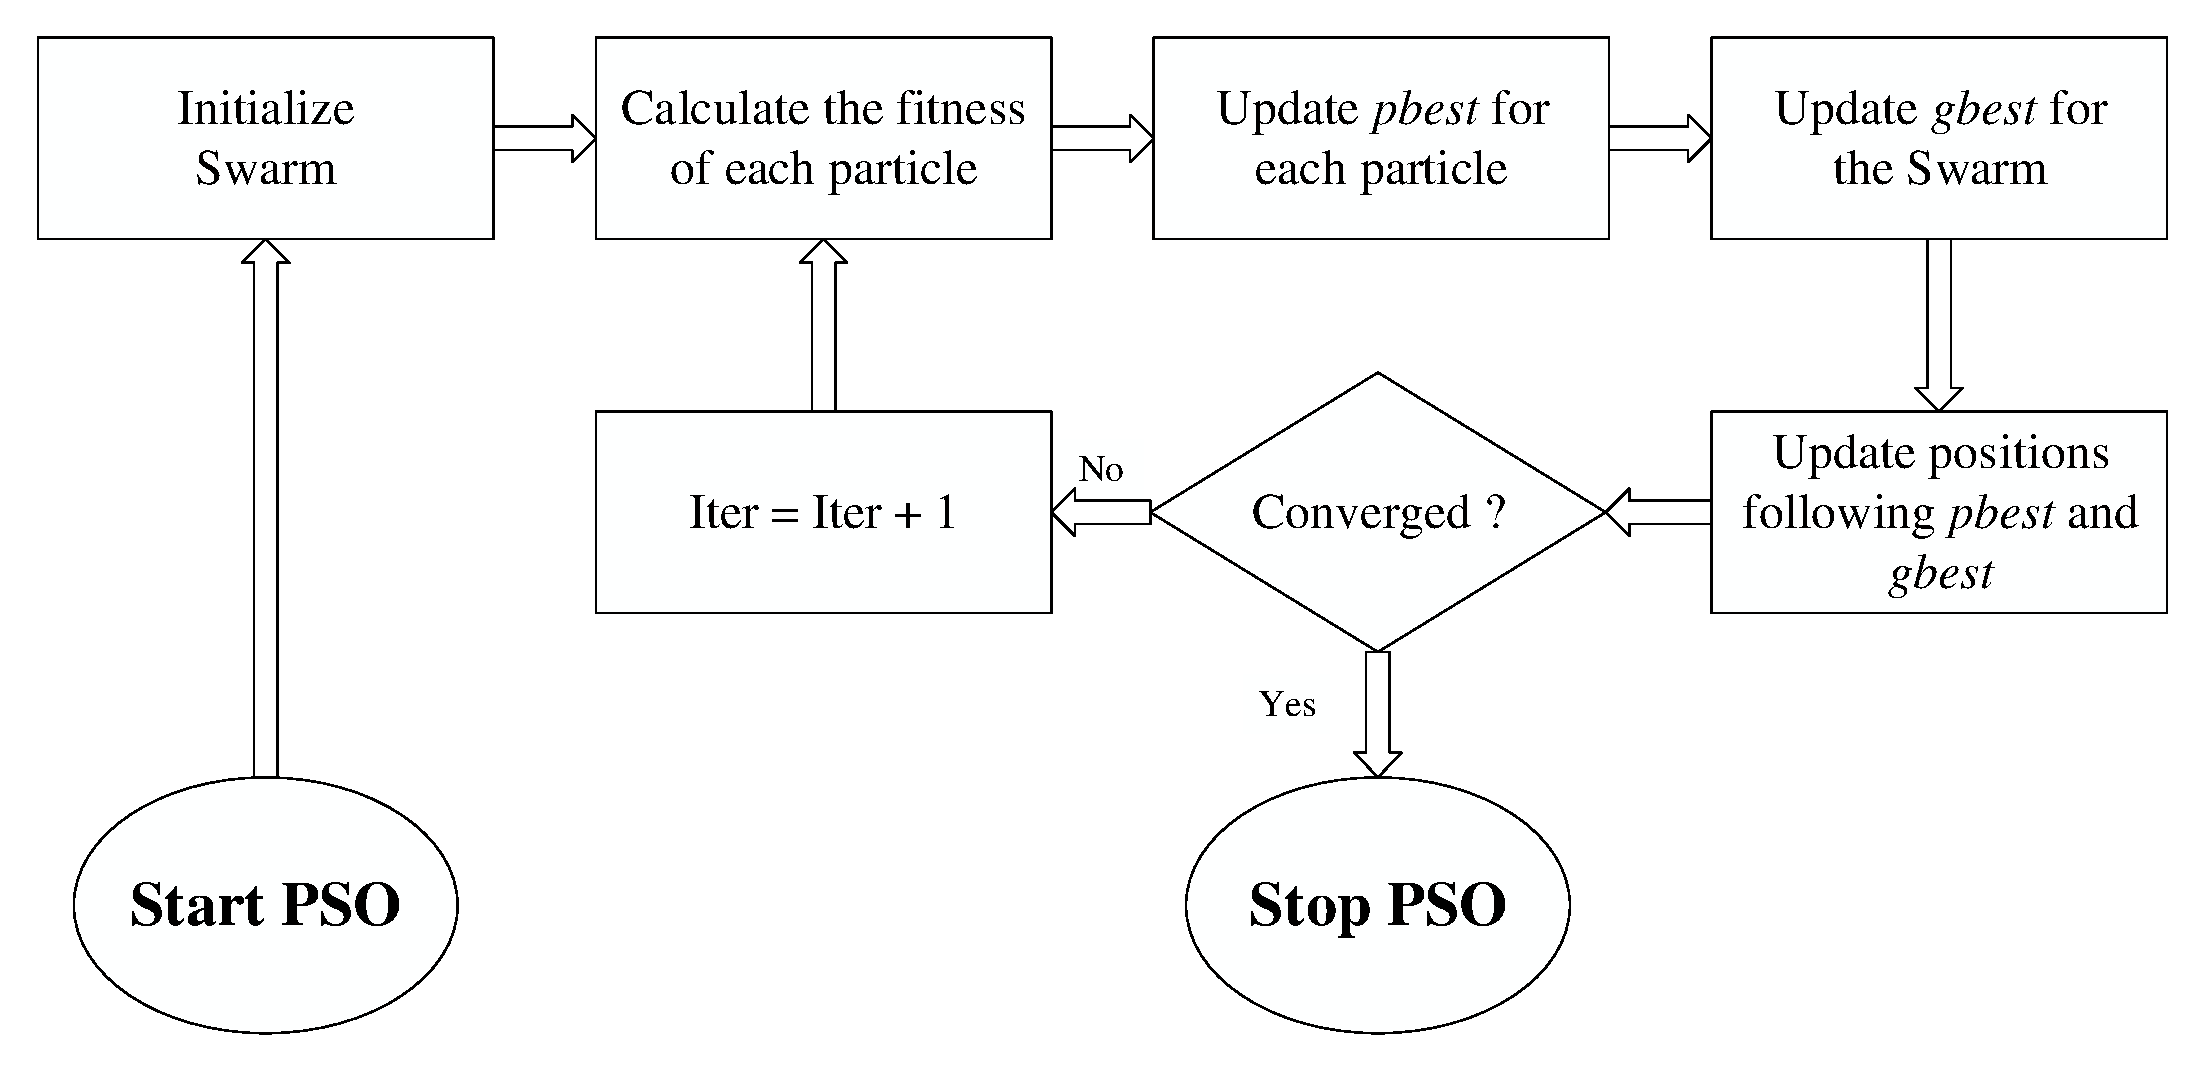
\includegraphics[width=0.75\linewidth]{pdf/model/pso}
  \caption{PSO flowchart} 
  \label{fig_pso_algo} 
\end{figure}
	 
Thus, each particle $i$ in swarm is described by two properties: its velocity $v_i$ and position $x_i$ in the search space. In each iteration, they are updated following the equation: 

\begin{equation} \label{eq_pso_1}
v_i^{t+1} = \omega.v_i^t + c_1.r_1(p_i^t - x_i^t) + c_2.r_2(g^t - x_i^t)
\end{equation}
\begin{equation} \label{eq_pso_2}
x_i^{t+1} = x_i^t + v_i^t
\end{equation}
where 
\begin{tabbing}
	xxx\=xxxxxxi\=\kill
	\>	$\omega$			\>	is inertia weight reduced linearly to zero through time; \\
	\>	$v_i^t$			\>	$v_i^t = [v_{i1}, v_{i2}, ..., v_{iD}]$ and is the velocity;	\\
	\>	$x_i^t$			\>	$x_i^t = [x_{i1}, x_{i2}, ..., x_{iD}]$ and is the position of 	\\
	\> 	\phantom{inv}	\> 	particle $i$ in current time $t$ respectively;\\
	\>	$p_i^t$			\>	is its personal best position in current time $t$; \\
	\>	$g^t$			\>	is global best position ever of entire swarm up to time $t$; \\
	\>	$c_1, c_2$ 		\>	are acceleration coefficients that pull particles \\
	\>	\phantom{inv} 	\>	faster to personal best and global best respectively;\\
	\>	$r_1, r_2$ 		\>	are random number which is uniformly distributed in $[0,1]$; \\
\end{tabbing}
\subsection{Sea Lion Optimization Algorithm (SLnO)}
\label{slno_standard} 

	Sea lions are considered as one of the most intelligent animals in wildlife which live on both lands and the oceans. They usually live in a large swarm with thousands of members, and this large swarm may contains many subgroups with their own hierarchy as well. In each subgroup, there is a dominant sea lion playing a role as the leader of the subgroup. All activities of subgroups are decided following the leader ship of that sea lion.
	
%	The most important characteristics of sea lions is that they have senses helping them to recognize and analyze immediately the movement of their prey such as fish even in the dark underwater environments. Like many predators, sea lions have their eyes point forward so that they can easily focus on the prey, but what makes their eyes different is that they can open pupils so widely to let much of light go through their eyes which helps them to see more clearly in underwater environment. Moreover, sea lions have their super-sensitive whiskers to locate exactly where the fish are. This can be done when the fish swim around, they leave waves or wakes behind them, and according to the intensity as well as the direction of waves, by using whiskers sea lions are able to detect and follow them.
	
	The intelligence of sea lions can be seen through the way they organize their groups and hunt the prey. Hunting as a group allow sea lions to have more opportunities of obtaining more food especially when the amount of fish is quite large. Usually, sea lions capture their prey together by circling the prey in a narrow ball, and the size of this "ball" continues to be decrease until the prey is totally wiped out. The main phases of hunting behaviors of sea lions can be illustrated as 3 steps as follows:
	
\begin{algorithm}[!t]
\caption{Sea Lion Optimization (SLnO)}
\label{algorithm_slno}
\SetAlgoLined
 Initialize the Sea Lion population $X_i (i=1,2,.., n)$ randomly. \\
 Calculate fitness of each solution (sea lion). \\
 $X_*\gets$ the best solution \\
\For {$Iter=0 \to Iter_{max}$}{
	Calculate the value of $C$ \\
	\For {SeaLion in population}{\
		Calculate $SP_{leader}$ using Eq. \ref{snlo_eq3}  \\
		\uIf{$SP_{leader} < 0.25$}{
			\uIf {$|C| < 1$}{\
				Update the location of the current search agent using Eq. \ref{slno_eq1}
				}
			\Else {
				Choose a random search agent $SL_{rand}$ \\
				Update the locatiion of current search agent by Eq. \ref{slno_eq8} \\
			}
		}	
		\Else{
			Update the location of the current search agent by Eq. \ref{slno_eq6}
		}
	Evaluate population: fix if any solutions go beyond the boundary \\
 	Recompute the fitness of all solutions \\
 	Check and update $X_*$ if a better solution is found. \\
	}
	
}
 \textbf{Results:}  $X_*, f(X_*)$
\end{algorithm}
	
\begin{itemize}
\item Tracking and chasing the prey using their senses.
\item Calling other members to gather and implement encircling strategy around the prey.
\item Attack towards the prey which is captured in the circle.
\end{itemize}

	Those behaviors is the inspiration for the Sea Lion Optimization (SLnO) which was first introduced in ~\cite{masadeh2019sea}. The algorithm mimics the amazing social behaviors and interesting hunting activities of sea lions. The formulas of the phases \textit{Detecting and tracking phase}, \textit{Vocalization phase} and \textit{Attacking phase} illustrate perfectly encircling mechanisms which is utilized by sea lions. We summarize and discuss briefly each phase in the algorithm as below, meanwhile the pseudo-code of SLnO is provided in details in \textbf{Algorithm \ref{algorithm_slno}}.

\begin{enumerate}
\item \textbf{Detecting and tracking phase}

	Sea lions can identify the location of the prey and gather other members that will join the subgroup to organize the net following the encircling mechanism. This sea lion plays an important role as a leader for this hunting behavior and other members' position will be updated following the position of the prey. In SLnO algorithm, the prey is considered as the current best solution or the solution closest to the optimal solution. This behaviors is presented mathematically using Eq. (\ref{slno_eq1}) and Eq. (\ref{slno_eq2}) as follows:
\begin{equation}\label{slno_eq1}
Dist = |2B.P(t) - SL(t)|
\end{equation}
\begin{equation}\label{slno_eq2}
SL(t+1) = P(t) - Dist.C
\end{equation}
	
	Where $Dist$ indicates the distance between the prey and the current sea lion; $P(t)$ and $SL(t)$ represent the position vectors of best solution and the sea lion in iteration $t$ respectively; $B$ is random vector in the range $[0, 1]$ which is multiplied by 2 to increase the search space, helping the search agent find optimal or near optimal position. $SL(t+1)$ is the new position of search agent after updating and $C$ is linearly decreased from 2 to 0 over the course of iterations, indicating the encircling mechanism of sea lion group when they move towards the prey and surround them.

\item \textbf{Vocalization phase}
	
	When a sea lion recognize a group of their prey (such as fish), it will call other sea lions in their group for gathering and creating a net to capture the prey. That sea lion is considered as the leader and it will lead the group of sea lions moving towards and decide the behaviors of the group. These behaviors are modeled mathematically as shown in Eq. (\ref{snlo_eq3}), (\ref{snlo_eq4}) and (\ref{snlo_eq5}):
\begin{equation}\label{snlo_eq3}
SP_{leader} = |(V_1(1+V_2)/V_2|
\end{equation}
\begin{equation}\label{snlo_eq4}
V_1 = \sin(\theta)
\end{equation}
\begin{equation}\label{snlo_eq5}
V_2 = \sin(\phi)
\end{equation}
 Where $SP_{leader}$ is the value that illustrates the decision of the leader followed by other sea lions in the group; $\theta$ and $\phi$ are the angles of its voice's reflection and refraction in the water, respectively.
 
\item \textbf{Attacking phase (Exploitation phase)}
 
 The hunting activities of sea lions are led by the leader. In SLnO algorithm, the target prey is considered the current best candidate solution. In order to mathematically mimic the hunting behaviors of sea lions, two phases are introduced as follows:
 	
\begin{itemize}
\item \textit{Dwindling encircling technique:}
	This behavior depends on the value of $C$ in Eq. \ref{slno_eq2}. $C$ is linearly decreased from 2 to 0 over the course of iterations, so this allows the search space around the current best position to shrink and force other search agents to updated in this search space as well. Therefore, a new updated position of a sea lion can be located anywhere in the search space between its current position and the location of the present best agent.

\item \textit{Circling updating position}: Sea lions chase bait ball of fishes and hunt them starting from edges. Eq. \ref{slno_eq6} is proposed in this regard:
\begin{equation} \label{slno_eq6}
SL(t+1) = |P(t) - SL(t)|.\cos(2 \pi m) + P(t)
\end{equation}	
\end{itemize}
	Where $|P(t) - SL(t)|$ illustrates the distance between the best optimal solution (the prey) and the current search agent in t-th iteration, $||$ means the absolute value and $m$ is a random number in the range $[-1, 1]$.
	
\item \textbf{Searching for prey (Exploration phase)}
	In exploration phase, the search agents update their positions based on a randomly selected sea lion. The condition that allows exploitation phase to happen is when the value of $C$ becomes greater than 1, and the process of finding a new agent is presented by Eq. (\ref{slno_eq7}) and (\ref{slno_eq8}) as below:
\begin{equation}\label{slno_eq7}
Dist = |2B.SL_{rnd}(t) - SL(t)|
\end{equation}
\begin{equation}\label{slno_eq8}
SL(t+1) = SL_{rnd}(t) - Dist.C 
\end{equation}  
Where $SL_{rnd}(t)$ is a random sea lion that is selected randomly from current population.

\end{enumerate}	

\section{Artificial Neural Network (ANN)}
\label{sec:ann}
\subsection{Activation functions}
\label{ann_act_func}

\begin{figure}[!ht] 
   \centering
   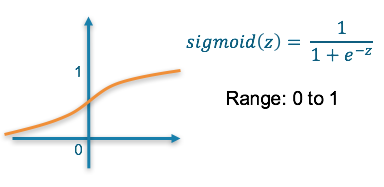
\includegraphics[width=0.33\linewidth]{png/sigmoid}
   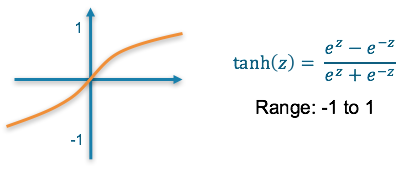
\includegraphics[width=0.33\linewidth]{png/tanh}
   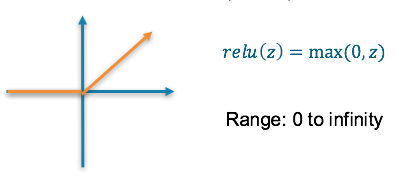
\includegraphics[width=0.33\linewidth]{png/relu}
   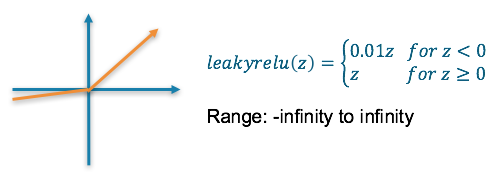
\includegraphics[width=0.33\linewidth]{png/leakyrelu}
  \caption{Activation functions. Source: https://medium.com/@srnghn/deep-learning-overview-of-neurons-and-activation-functions-1d98286cf1e4} 
  \label{fig_activation} 
\end{figure}

	Activation functions also known as transfer functions are used to map input nodes to output nodes in certain fashion. Activation functions are extremely important for an ANN to learn and figure out features and characteristics of data which need a non-linear transformation to become outputs. There are the four most popular functions used in Deep Learning, their names are Sigmoid, Hyperbolic Tangent (Tanh), Rectified Linear Units (ReLU), Leaky ReLU and Exponential Linear Unit (ELU) (See in Fig. \ref{fig_activation}).

\begin{itemize}
\item \textbf{Sigmoid function}: takes a number as input and returns a value in $	[ \,0,1] \,$.
	$$f(x) = \frac{1}{1+e^x}$$
\item \textbf{Hyperbolic Tangent (Tanh) function}: is also like Sigmoid function but better, the range of the output from Tanh funtion is in $	[ \,-1,1] \,$.
 $$f(x) = \frac{2}{1+e^{-2x}} = 2\sigma(2x)-1$$
\item \textbf{Rectified Linear Unit (ReLU) function}: is a function having threshold at $0$ value. It helps accelerate the training process in ANN, so it is used in almost all the complicated deep learning models such as RNNs and CNNs.
$$f(x) = max(0, x)$$
\item \textbf{Leaky ReLU function}: is like ReLU function, but instead of setting thresholf value at $0$, Leaky ReLU extends the domain to $\alpha x$.
\[
    f(x)= 
\begin{cases}
    x,& \text{if } x > 1\\
    \alpha x, & \text{otherwise}
\end{cases}
\]
\end{itemize}
	
\subsection{Loss functions}
\label{ann_loss_func}
Neural Networks are trained by backpropagation algorithm, which updates the weights parameters of ANN according to a loss value. The loss value is calculated by a loss function, so loss functions are totally vital when an ANN model is built for learning information from data. These functions will essentially measure how poorly a model is performing by comparing what the model is predicting with the actual value it is supposed to output. Therefore, choosing a loss function that is appropriate for penalizing model effectively is one of the most important tasks while working with data. There are a number of loss functions for deep learning models, and each of them have its own pros and cons. The common loss functions that are widely used in time-series forecasting will be presented as below:
\begin{itemize}
\item  \textbf{Mean Absolute Error (MAE)}: 
$$MAE = \frac{\sum|e_t|}{N}$$
\item  \textbf{Sum Square Error (SSE)}: $$SSE = \sum(e_t^2)$$
\item  \textbf{Mean Square Error (MSE)}: $$MSE = \frac{\sum(e_t^2)}{N}$$
\item  \textbf{Root Mean Square Error (RMSE)}: $$RMSE = \sqrt{MSE}$$
\item  \textbf{Mean Absolute Percentage Error (MAPE)}: $$MAPE = \frac{1}{N}\sum|\frac{e_t}{y_t}|$$
Where $N$ is the number of data points, $y_t$ is the actual output value, $d_t$ is the output value predicted by models, $e_t = d_t - y_t$ is the error value of the data point $t$.
\end{itemize}
	 
\subsection{Backpropagation - the ANN Training Algorithm}
\label{ann_backprop_alg}

\begin{algorithm}[!t]
	\caption{Backpropagation algorithm applied for FFNN with 1 hidden layer}
	\label{algorithm_backprop}
	\SetAlgoLined
	Initialize randomly weights' value $w_p$\\ 
	\Repeat{Until convergence or the number of iterations is enough}{
	\textbf{Calculate output value(s) according to weights and input}  \\
	
		\For{$j= 1$ to $h$}
		{
			$H_{j} = \phi(\sum_i^n {x_i*w_{ij}^{[1]} + b_{ij}^{[1]}})$ \\ 
			
		}
		$\widehat {{y_j}} = \phi(\sum_i^h{H_i * w_j^{[2]} + b_j^{[2]}})$\\
		
		\textbf{Calculate Loss value by loss function} \\ 
		
		$L(w) = loss(\widehat {{y_j}},{y_j})  $ \\
		
		 \textbf{Backpropagating Loss to weights}\\
		
		$ \bigtriangleup(w_{ij}^2) = \frac{\partial (L(w))}{\partial (w_{ij}^2)}$ \\
		$ \bigtriangleup(w_{ij}^1) = \frac{\partial (L(w))}{\partial (w_{ij}^1)}$ \\
		
		\textbf{Update weights' value} \\ 
		
		$w_{ij}^2 = w_{ij}^2 - \eta * \bigtriangleup(w_{ij}^2)$ \\
		$w_{ij}^1 = w_{ij}^1 - \eta * \bigtriangleup(w_{ij}^1)$
	}
		
\end{algorithm}

Back-propagation algorithm is undoubtedly the most fundamental building block in an ANN. It It was first introduced in 1960s and almost 30 years later (1989) popularized by Rumelhart, Hinton and Williams in~\cite{rumelhart1988learning}. The algorithm is used to effectively train a neural network through a method called chain rule. In simple terms, after each forward pass through a network (propagation phase), back-propagation performs a backward pass while adjusting the model\textquotesingle s parameters (weights and biases) (weights updating phase).

\subsubsection{Forward propagation phase}
\begin{enumerate}
\item The input values will be fed into ANN through input layer, going forward to hidden layers, and finally to output layer, creating predicted output values. While propagation process, each layer uses its own activation function (sec. \ref{ann_act_func})
\item Error values are calculated by the loss function and propagated back to previous layers.
\end{enumerate}
\subsubsection{Weights updating phase}

\begin{enumerate}
\item Calculating gradients of loss function in weights and biases following the chain rule.
\item Updating weights and biases is done according to gradients' values 
\end{enumerate}

These two phases are repeated in each iteration during training. The algorithm will be stopped when the error from loss function reach a acceptable value or when the training iteration is large enough. The algorithm\textquotesingle s pseudo code is presented in short in Algorithm \ref{algorithm_backprop}.

\section{Time-series prediction and Auto-scaling problem in Cloud Computing}
\label{sec:application}

\subsection{Cloud Computing}
\label{cloud}

\subsection{Auto-scaling problem}
\label{auto_scale}

\subsection{Well-known machine learning models for Auto-scaling in cloud computing}
\label{wl_known_models}

	Recent developments in cloud computing including resource management have resulted in a significant interest in resource usage prediction . Various methods have been proposed for solving this problem with different aspects, objectives and applications ~\cite{amiri2017survey}. In this section, we focus on several Artificial Neural Network (ANN) models that are used for tackling the time-series characteristic in resource usage forecast in cloud computing environment.
	Deep Feed-forward Neural Network, also called Feed-forward Neural Network (FFNN) are the quintessential deep learning models. The goal of all FFNN is to approximate some functions $f^*$.  In Regression problems, $y = f^*(x)$ maps an input $x$ to a value $y$. A feed-forward network defines a mapping $y = f(x,\theta)$ and learns the value of the parameters $\theta$ that result in the best function approximation. ~\cite{Goodfellow-et-al-2016}. These models are called feed-forward because information flows through the function being evaluated from $x$, through the intermediate computations used to define $f$, and finally to the output $y$. There are no feedback connections in which outputs of the model are fed back into itself. When feed-forward neural networks are extended to include feedback connections, they are called recurrent neural networks, which will be discussed in ~\ref{model_rnn}.
	
	In general, Multi-Layer Perceptrons (MLPs) models contain several disparate layers. The first layer is input layer taking information $x$ as input for the network. The last layer is called output layer, whose value is the result of $y$ with input $x$. The layers between the input and output layers are hidden layers. The structures of hidden layers are extremely diverse, varying from model to model. As presented in Fig. \ref{fig_model_mlp}, a hidden layer of a simple FFNN is a group of neurons with no connection to each other, while in Recurrent Neural Networks (RNN), and Convolution Neural Network (CNN) hidden layer is a recurrent layer, and convolution layer respectively. 
	
	The Deep Neural Networks that are applied for Time series prediction will have input neurons presenting the historical data. The models utilize information from data in the past for forecasting future data. Input data presented as $x_1, x_2, ..., x_t$ is considered as historical values up to time t, which is used to predict the value at the time $t+1$. In other words, Deep Neural Networks will learn from data and approximate a function transforming the historical data up to time $t$ to the data at the time $t+1$ as follows:
\begin{equation} \label{eq_ffnn_1}
x(t+1) = y = f(x_1, x_2, ..., x_t)
\end{equation}
	
	 In this section, we summarize several Deep Neural Network models, which are widely used for time series forecasting. They are simple Multi-Layer Perceptrons (MLPs), Cascade Forward Neural Network (CFNN) and Recurrent-based Neural Network including traditional Recurrent Neural Network (RNN), Long-Short Term Memory (LSTM) and Gated Recurrent Units (GRU). Each method will be presented below with brief ideas and mathematical formulas. 

\begin{figure}[!ht] 
   \centering
   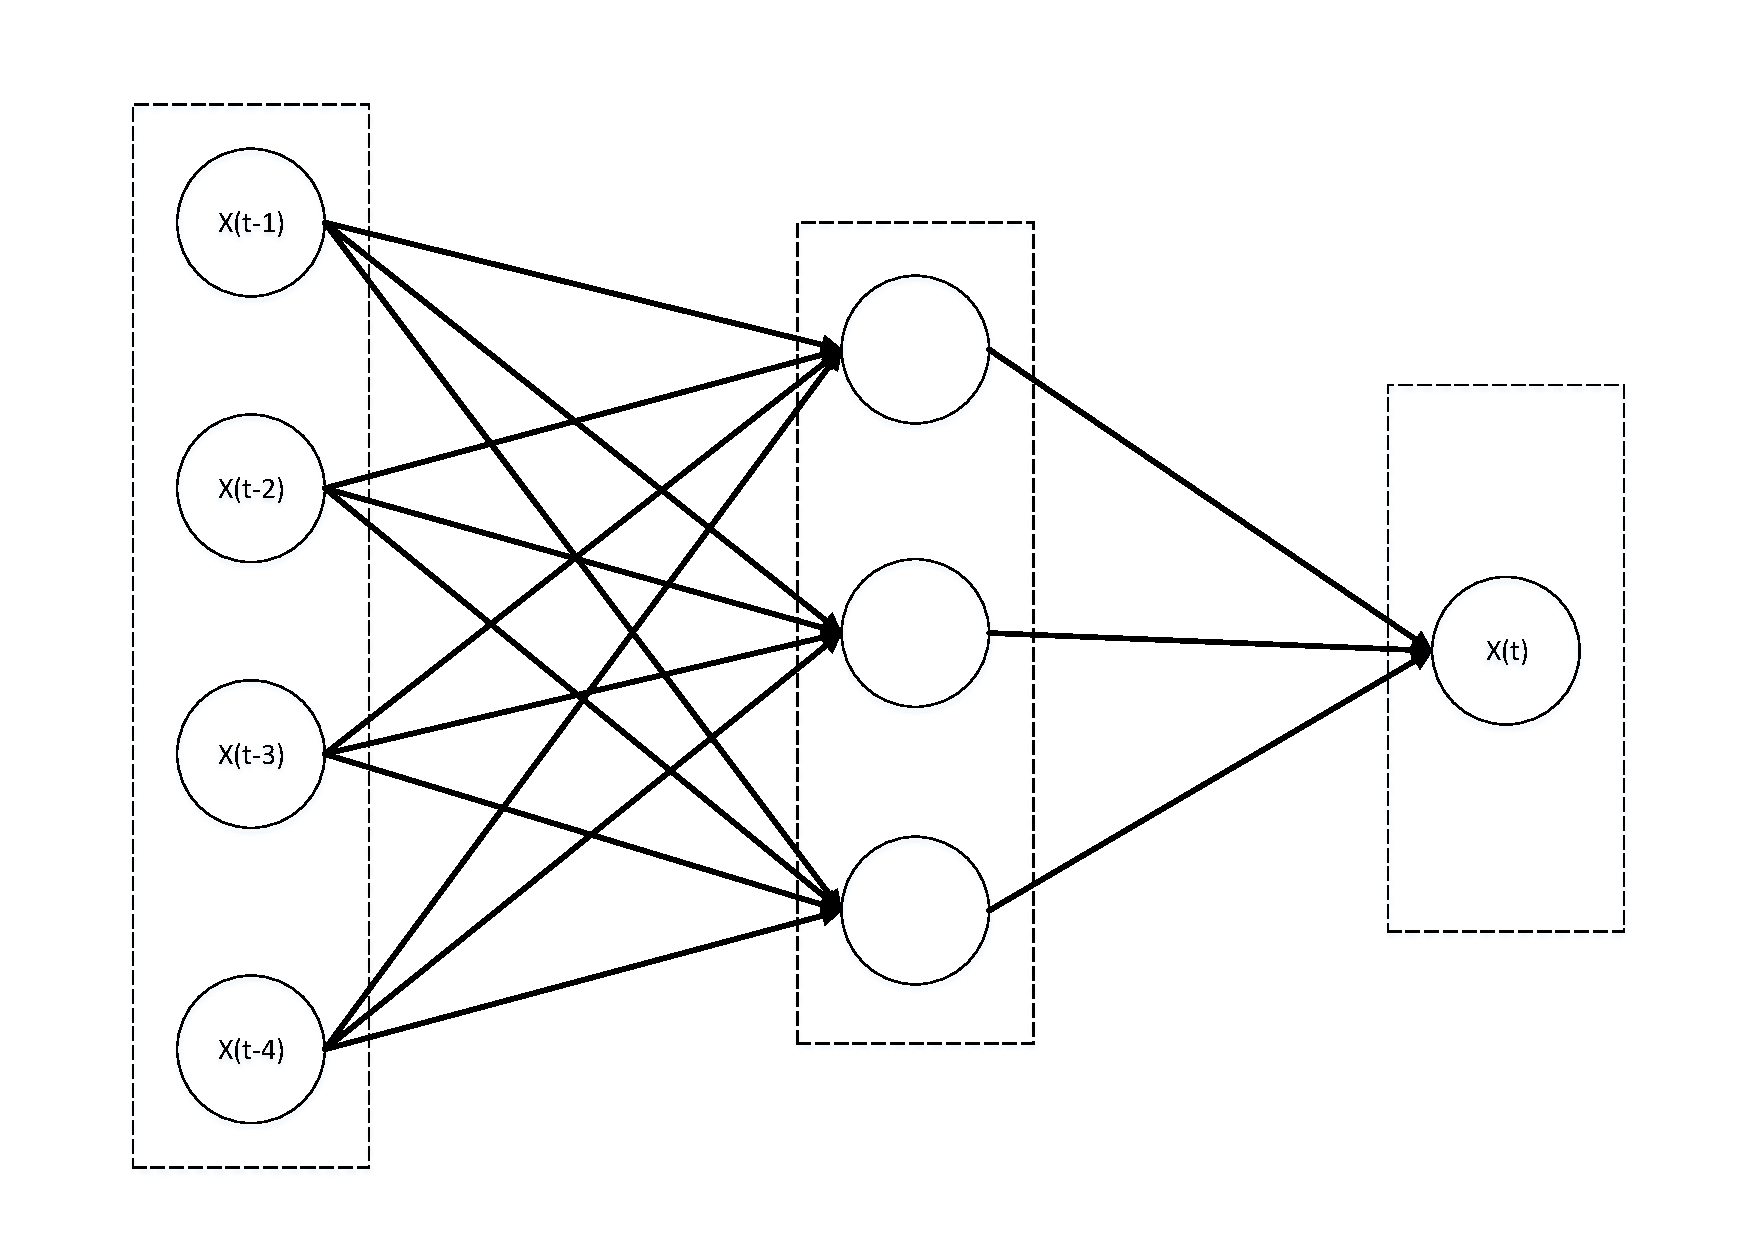
\includegraphics[width=0.75\linewidth]{pdf/model/model_ffnn}
  \caption{An example of MLPs model in time-series prediction.} 
  \label{fig_model_mlp} 
\end{figure}

\subsubsection{Multi-Layer Perceptrons (MLPs)}
\label{model_mlp}
	
	The additional layers added between input layer and output layer make network architecture contain hidden layers and called Multi-Layer Perceptrons (MLPs). The input data is fed through input layer to hidden layers in the weighted form. The information from input data $X$ is distributed to the neurons in hidden layers and then processed by an activation function. The activation function in hidden layers are non-linear function playing a role as a transfer function, helping MLPs learn non-linear characteristics of the data. The information after being processed by hidden layers then are sent to output layer in the weighted sum, and also go through an activation function as well, creating the output value $y$. MLPs model is used in predicting time series data ~\cite{azoff1994neural}, ~\cite{koskela1996time}.  Fig. \ref{fig_model_mlp} shows a MLPs with a 4-neuron input layer and one output layer. In general,  the mathematical equation of the MLPs architecture can be written as follows:
\begin{equation} \label{eq_mlp_1}
H = f_h(W_h^TX + b_h)
\end{equation}
\begin{equation} \label{eq_mlp_2}
y = O = f_o(W_o^TH + b_o
\end{equation}

Where $X$ is the input data, $H$ and $O$ are the information after being fed through the hidden and output layers. $W_h$, $b_h$ and $W_o$, $b_o$ are weights and biases, while $f_h$ and $f_o$ are activation functions of hidden layer and output layer, respectively.


\subsubsection{Cascade Forward Neural Network (CFNN)}
\label{model_cfnn}

The main difference between CFNN and MLPs is that in CFNN, perceptron connection is added directly between neurons in input layer and output layer, while in MLPs, that connection is indirect through the hidden layer. The output layer of CFNN perceives both transformed information that is output of hidden layer, and the raw information from input data. This Deep Neural Network model was first used for forecasting monthly palm oil price in the Europe market in ~\cite{warsito2018cascade}. The architecture of CFNN with 4-neuron input layer is illustrated in Fig. \ref{fig_model_cfnn}, and the mathematical formulas for CFNN model are presented as follows:
\begin{equation}\label{eq_cfnn_1}
H = f_h(W_h^TX + b_h)
\end{equation}
\begin{equation}\label{eq_cfnn_2}
C = f_c(W_c^TX) + b_c
\end{equation}
\begin{equation}\label{eq_cfnn_3}
y = O = f_o(W_o^TH + b_o) + C
\end{equation} 
where $f_c$ is the activation function from the input layer to output layer, $C$ is the output value of $f_c$, and $W_c, b_c$ are weights and biases of the connection, respectively.

\begin{figure}[!ht] 
   \centering
   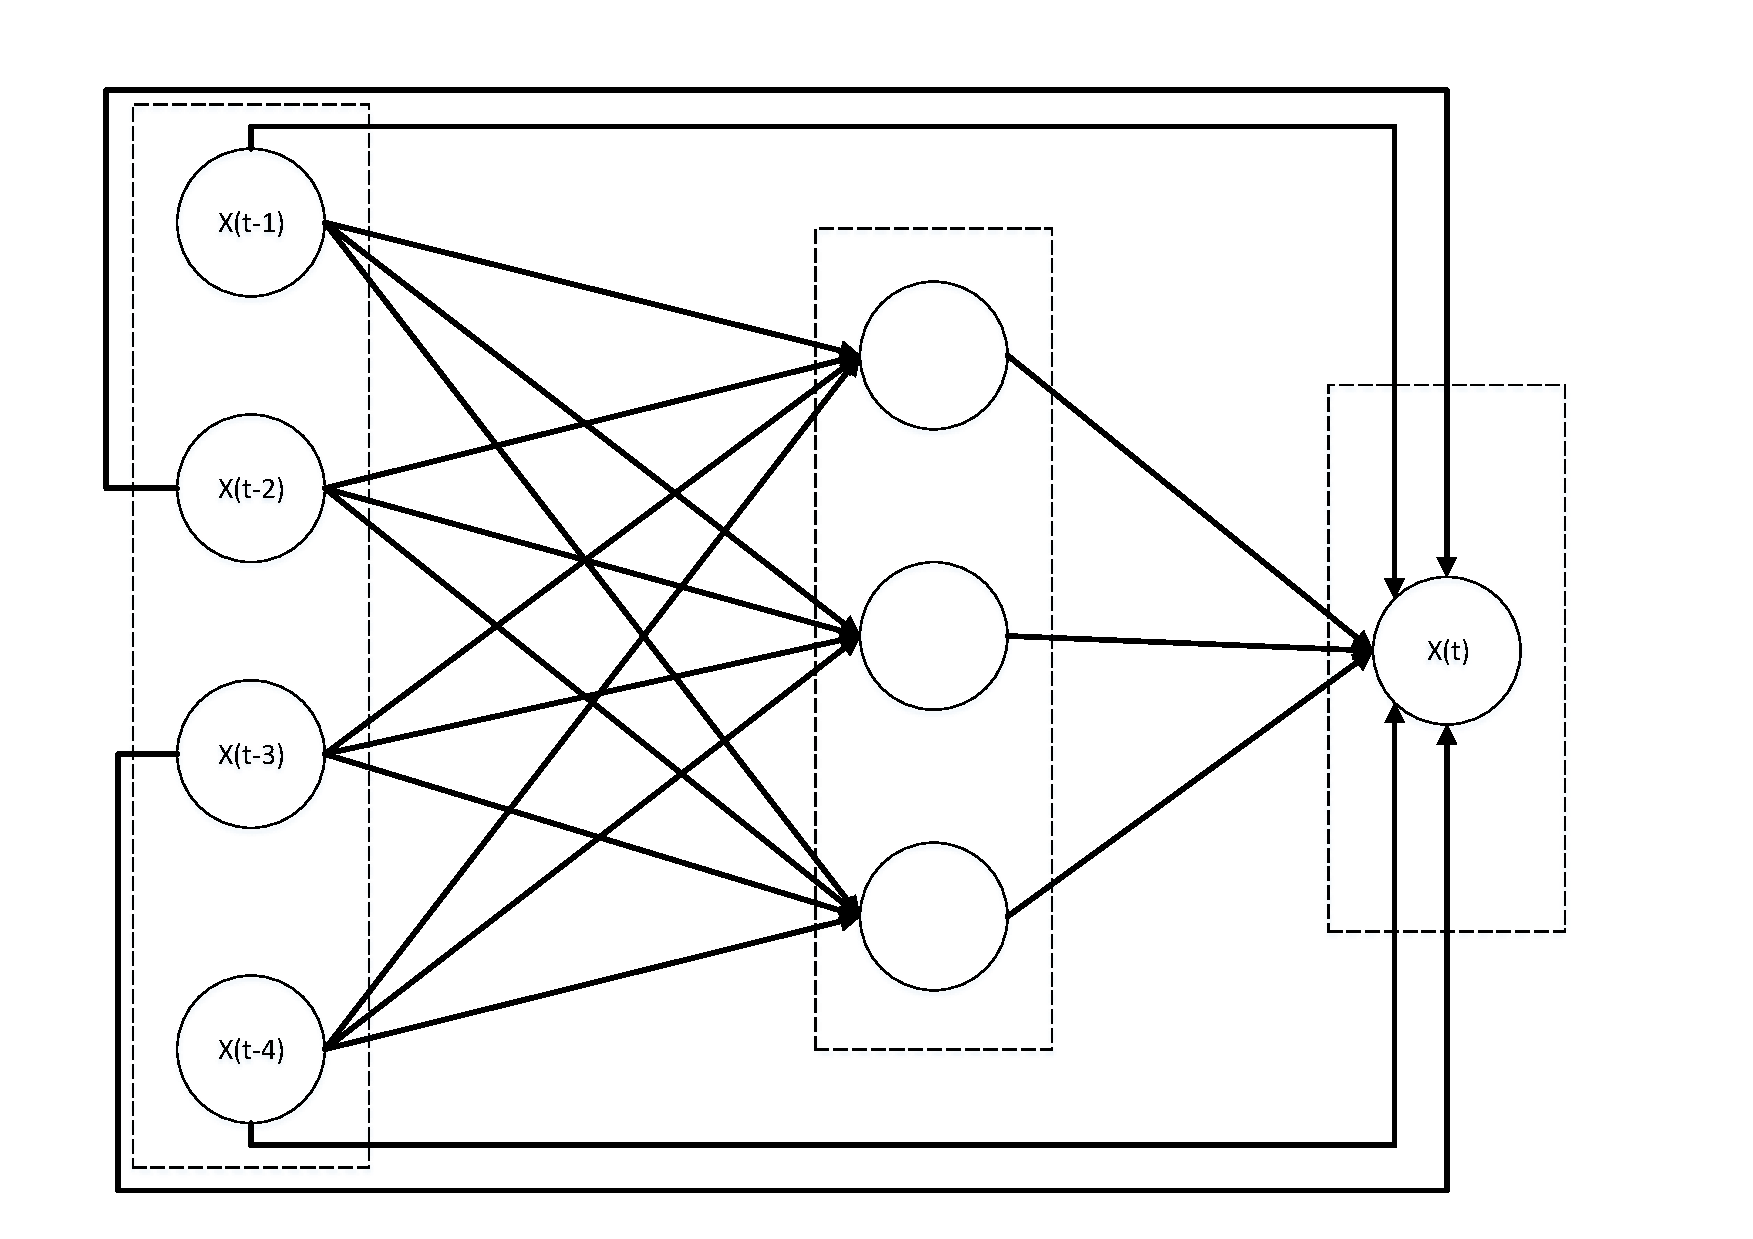
\includegraphics[width=0.75\linewidth]{pdf/model/model_cfnn}
  \caption{An example of CFNN model in time-series prediction.} 
  \label{fig_model_cfnn} 
\end{figure}


\subsubsection{Recurrent Neural Network (RNN)}
\label{model_rnn}
	Recurrent neural networks (RNNs) are dynamical systems that are specifically designed for temporal problems, as they have both feed-back and feed-forward connections (Fig. \ref{model_rnn}). RNN remembers the past and  its decisions are influenced by what it has learned from the past. RNNs can take one or more input vectors and produce one or more output vectors and the output(s) are influenced not just by weights applied on inputs like a regular MLPs, but also by a state vector representing the context based on prior input(s)/output(s),  so the same input could produce a different output depending on previous inputs in the series. For that reason, RNN is one of the most popular models being used for modeling time series data~\cite{zhang2000predicting},~\cite{connor1994recurrent},~\cite{chandra2012cooperative}. There are two popular and efficient RNN models that work really well: Long Short-Term Memory (LSTM) and Gated Recurrent Unit (GRU) which are discussed below. 
\begin{figure}[!ht] 
   \centering
   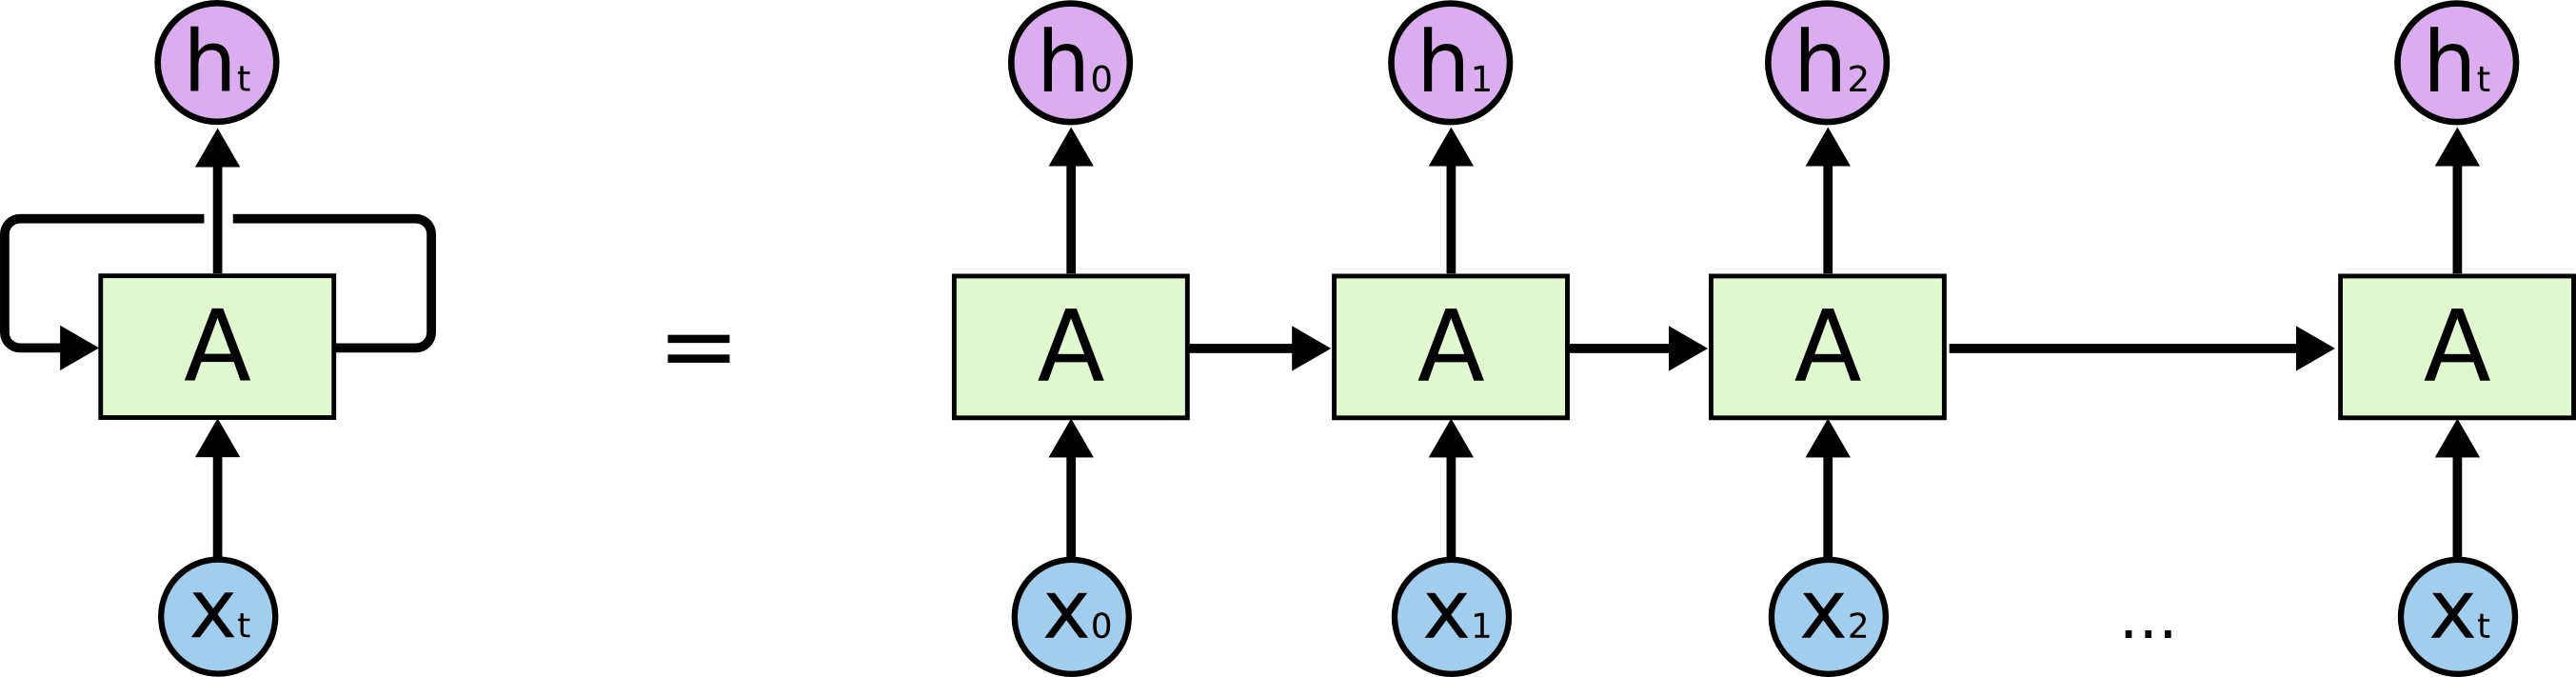
\includegraphics[width=1.0\linewidth]{png/rnn_unrolled}
  \caption{Traditional RNN architechture. Source: https://colah.github.io/posts/2015-08-Understanding-LSTMs/} 
  \label{model_lstm_gru} 
\end{figure}

\subsubsection{Long Short-Term Memory (LSTM)}
	Long short-term memory (LSTM)~\cite{hochreiter1997long} is a special kind of RNN created for learning long-term dependencies. LSTM units have 3 gates managing the contents of the memory. These gates are simple logistic functions of weighted sums, where the weights might be learnt by backpropagation. It means that, even though it seems a bit complicated, the LSTM perfectly fits into the neural network and its training process. With combining a forget gate in LSTM units, LSTM is capable to determine what it needs to remember and forget, so LSTM can work very well with dependent data , especially with time series data ~\cite{gers2002applying}, ~\cite{guo2016robust}, ~\cite{fu2016using}. The architecture of LSTM units is illustrated in Fig. \ref{model_lstm_gru}, and its mathematical model is briefly described as follows:
	 The input gate (\ref{eq_lstm_1}) and the forget gate (\ref{eq_lstm_2}) manage the cell state (\ref{eq_lstm_4}), which is the long-term memory. The output gate (\ref{eq_lstm_3}) produces the output vector or hidden state (\ref{eq_lstm_5}), which is the memory focused for use. This memory system enables the network to remember for a long time, which was badly missing from vanilla recurrent neural networks. 
\begin{equation}\label{eq_lstm_1}
i_t = sigmoid(W_ix_t + U_ih_{t-1}+b_i)
\end{equation}
\begin{equation}\label{eq_lstm_2}
f_t = sigmoid(W_fx_t + U_fh_{t-1}+b_f)
\end{equation}
\begin{equation}\label{eq_lstm_3}
o_t = sigmoid(W_ox_t + U_oh_{t-1}+b_o)
\end{equation}
\begin{equation}\label{eq_lstm_4}
c_t = f_t \odot c_{t-1} + i_t \odot tanh(W_cx_t + U_ch_{t-1} + b_c)
\end{equation}
\begin{equation}\label{eq_lstm_5}
h_t = o_t \odot tanh(c_t)
\end{equation}
\begin{figure}[!ht] 
   \centering
   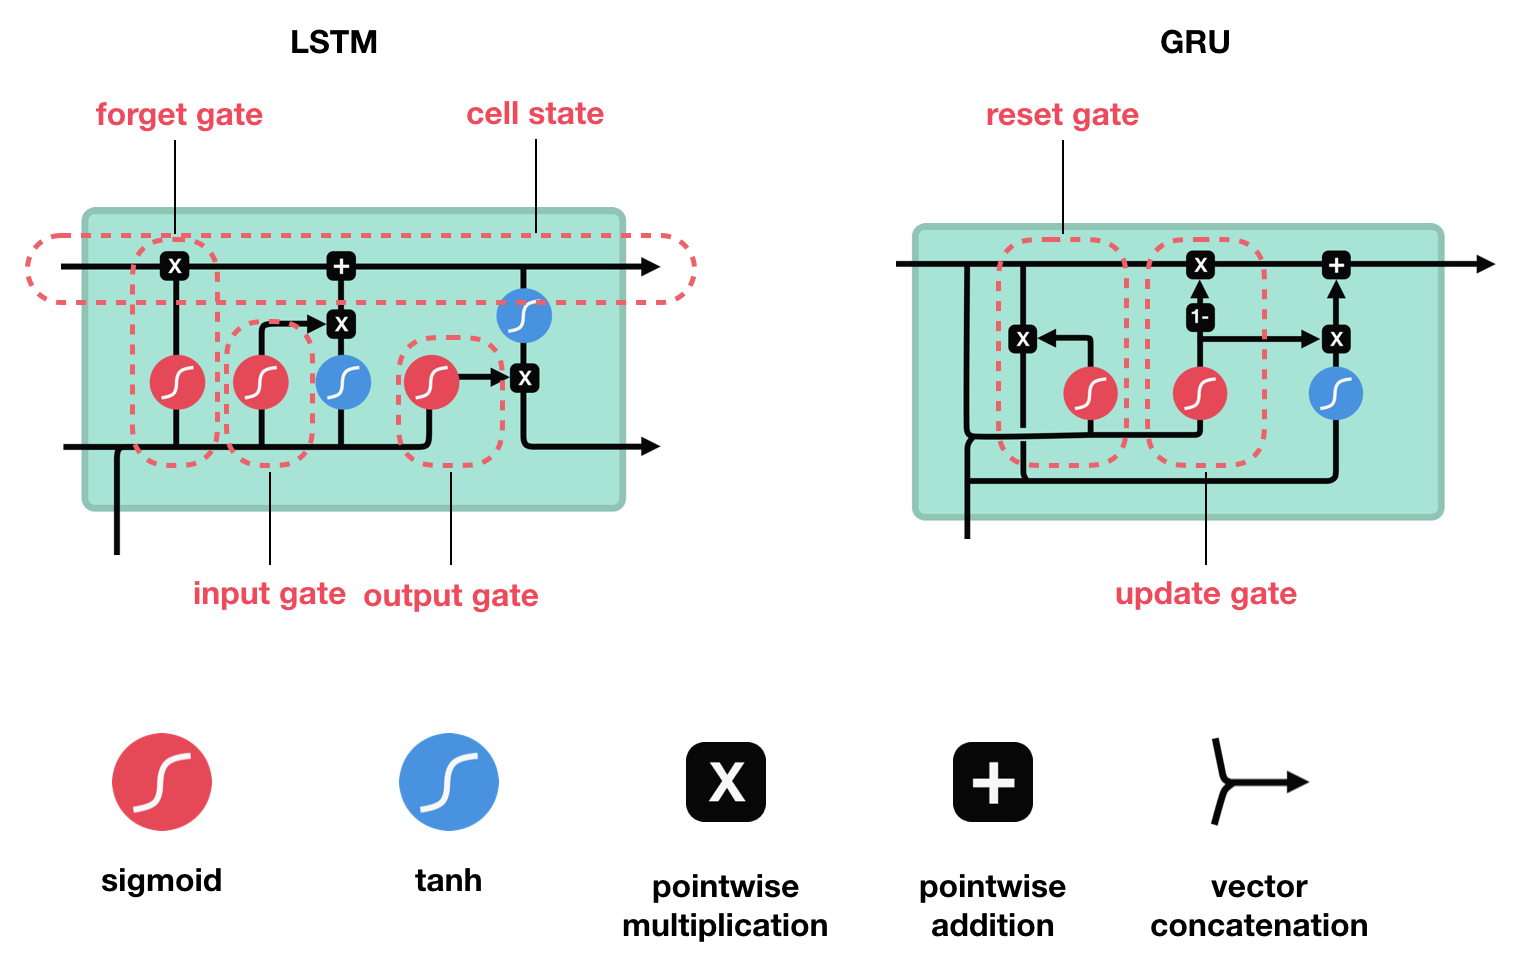
\includegraphics[width=1.0\linewidth]{png/lstm_gru}
  \caption{LSTM and GRU architechture. Source: https://towardsdatascience.com/illustrated-guide-to-lstms-and-gru-s-a-step-by-step-explanation-44e9eb85bf21} 
  \label{model_lstm_gru} 
\end{figure}

\subsubsection{Gated Recurrent Units (GRU)}

	Gated recurrent unit (GRU)~\cite{chung2014empirical} is essentially a simplified LSTM. Different form LSTM, GRU uses two gated called update gate and reset gate. Basically, these gates are two vectors managing what information should be passed to the output. In GRU, its gates can be trained to keep information from long ago, without washing it through time or remove information which is irrelevant to the prediction. It has the exact same role as LSTM in the network. The main difference is in the number of gates and weights - GRU is somewhat simpler. Like LSTM, GRU is also a widely chosen solution for time series forecasting such as in~\cite{langkvist2014review} and~\cite{bone2000recurrent} The srtucture of GRU units is presented in Fig. \ref{model_lstm_gru} following the mathematical model as below:
	
	The update gate~\ref{eq_gru_1} controls the information flow from the previous activation, and the addition of new information as well~\ref{eq_gru_3}, while the reset gate~\ref{eq_gru_2} is inserted into the candidate activation. Overall, it is pretty similar to LSTM. From these differences alone, it is hard to tell, which one is the better choice for a given problem. 
\begin{equation}\label{eq_gru_1}
z_t = sigmoid(W_zx_t + U_zh_{t−1} + b_z)
\end{equation}
\begin{equation}\label{eq_gru_2}
r_t = sigmoid(W_rx_t + U_rh_{t−1} + b_r)
\end{equation}
\begin{equation}\label{eq_gru_3}
h_t = z_t\odot h_{t-1} + (1 - z_t)\odot tanh(W_hx_t + U_h(r_th_{t-1}) + b_h)
\end{equation}


\chapter{Improved Sea Lion Optimization (ISLO) algorithm and Proposed Model for Auto-Scaling (ISLO-CFNN)}
\section{Improved Sea Lion Optimization (ISLO)}
\label{improved_ISLO}
	Sea Lion Optimization (SLnO) is one of the newest swarm-based optimization algorithm. In experiments in SLnO original paper \cite{masadeh2019sea}, SLnO is proved that it outperformed several well-known bio-inspired model such as Generic Algorithm (GA), Particle Swarm Optimization (PSO) and Whale Optimization Algorithm (WOA). However, like many other algorithms, SLnO also faces the problem of local minimum, slow convergence and diversity degradation of population. In SLnO's exploitation phase, the updating operation \ref{slno_eq2} only takes the distance between the current agent and the best solution into account, which makes updated position always oriented to one direction, leading to poverty of exploitation ability. Also, in exploration phase, although the participation of two agents that already exist in population in the updating operation \ref{slno_eq8} helps the new-born solution inherits current decent features of population, new solution has no way to reach another position outside of existing positions. This results in a dramatic decrease in the diversity of population, and significantly influences the ability of escaping local minimum of SLnO algorithm. All things considered, we decided to enhance those 2 operators by taking individual information into account for exploitation phase, and using a technique called opposition-based operation for exploration phase. These two improvements form a new version of SLnO called Improved Sea Lion Optimization (ISLO) algorithm. The pseudo code of the algorithm is presented in Algorithm \ref{algorithm_islo}, and  our improvements would be discussed in detail in \ref{imprv_exploit} and \ref{imprv_explore} as below.  
\begin{algorithm}[!t]
\caption{Improved Sea Lion Optimization (ISLO)}
\label{algorithm_islo}
\SetAlgoLined
 Initialize the Sea Lion population $X_i (i=1,2,.., n)$ randomly. \\
 Calculate fitness of each solution (sea lion). \\
 $X_*\gets$ the best solution \\
\For {$Iter=0 \to Iter_{max}$}{
	Calculate the value of $C$ \\
	\For {SeaLion in population}{\
		Calculate $SP_{leader}$ using Eq. \ref{snlo_eq3}  \\
		\uIf{$SP_{leader} < 0.25$}{
			\uIf {$|C| < 1$}{\
				Calculate $Dist_1$ and $Dist_2$ using Eq. \ref{islo_eq1} and \ref{islo_eq2}
				Update the location of the current search agent using Eq. \ref{islo_eq3}
				}
			\Else {
				Choose a random search agent $SL1_{rand}$ and $SL2_{rand}$ \\
				Update the location of current search agent by Eq. \ref{islo_eq4} \\
			}
		}	
		\Else{
			Update the location of the current search agent by Eq. \ref{slno_eq6}
		}
	Evaluate population: fix if any solutions go beyond the boundary \\
 	Recompute the fitness of all solutions \\
 	Check and update $X_*$ if a better solution is found. \\
	}

}
 \textbf{Results:}  $X_*, f(X_*)$
\end{algorithm}   
\subsection{Exploitation phase improvement}
\label{imprv_exploit}
	As mentioned above, SLnO have its own drawbacks in its exploitation phase. In order to enhance the performance of the operation \ref{slno_eq2}, not only distance between the current agent and the best agent, but also the influences of an individual experiment in history is considered in new improved operation. This idea stems from the updating mechanism of PSO \cite{eberhart1995particle} where the velocity of a particular particle is influenced by both the best individual and best personal information. ***************.
	
	Following that idea, we apply the information sent from best individual experiment in the same way as best agent position. The formulas of new updating mechanism for exploitation phase is as follows:
\begin{equation}\label{islo_eq1}
Dist_1 = |2B.P(t) - SL(t)| 
\end{equation}
\begin{equation}\label{islo_eq2}
Dist_2 = |2B.P_i(t) - SL(t)| 
\end{equation}
\begin{equation}\label{islo_eq3}
SL(t+1) = c_1r_1(P(t) - Dist_1.C) + c_2r_2(P_i(t) - Dist_2.C)
\end{equation}
where $P_i(t)$ is the personal best position of agent $i$ up to time $t$, $c_1$, $c_2$ 2 are positive constant parameters called acceleration coefficients and $r1, r2$ are random numbers in range $[\, 0,1 ] \,$.

	In new operation \ref{islo_eq3}, the new-updated position of an individual is the result of adding two vectors, one is the vector presenting the direction of that individual towards the best agent, and another is the direction towards its own experiences in history. The influences of both two factors are determined by two random numbers $r_1$ and $r_2$. $r_1$ and $r_2$ play an extremely important role in the updating mechanism,  because  they create random characteristics for the operation, helping ISLO avoiding local minimum and taking advantages of the two factors. Without the appearance of $r_1$ and $r_2$, the updated position is always affected exactly half by best agent and half by its experience, which may lead to degradation of the diversity of population. 

\subsection{Exploration phase improvement}
\label{imprv_explore}
	
	In original SLnO algorithm, new-born agents that are created in exploration phase cause a poor exploration search ability because of inheriting features of existing solutions. In order to tackle this problem, exploration phase is required the operation to have the ability of creating a decent new-born solution. New updated position need to satisfy two characteristics: carrying random features for ensuring a strong capability of exploration phase, and landing in a position decent enough (close enough to the best agent position) for updating positions in the next generation. From that motivation, a method called Opposition-based Learning (OBL) \cite{tizhoosh2005opposition}, which is successfully applied for enhancing bio-inspired optimization algorithms such as GA \cite{tizhoosh2005opposition}, PSO \cite{wang2007opposition} \cite{tang2009enhanced} in solving several optimization problems including finding parameter for deep learning models \cite{rashid2010improved} \cite{nguyen2019efficient} is utilized as a base model for our improvement in exploration operation of SLnO. 
	
	
	The idea of OBL is applied in the operation in the way of finding a new random optimal solution, but still retain a part of features from existing solutions. This is done by calculating the opposed position to the current position of an living agent in population. For ensuring random characteristics of new found position, a random agent from population, and a random agent in the search space will be chosen for participating in this operation. The mathematical formulas are given as follows:
\begin{enumerate}
\item Select a random solution $SL1_{rand}$ in the search space.
\item Select a random existing solution $SL2_{rand}$ in the population.
\item Create a new solution $SL_{rand}$ by calculating the opposed position to $SL1_{rand}$ through $SL2_{rand}$.
\begin{equation} \label{islo_eq4}
SL_{rand} = 2*SL2_{rand} - SL1_{rand}
\end{equation}
\end{enumerate}

\section{Proposed model for auto-scaling problem in Cloud Computing}
\label{sec:proposed_model}
	
	In chapter \ref{ch:background}, we generally discussed about Cloud Computing and the problem of auto-scaling with the existing methods for solving this. In general, it is relatively necessary to build cloud computing servers with the capacity of automatically expanding and  shrinking the resources allocated. Although there are a number of solutions proposed for tackling this issue, they all have their own drawbacks.
	
	The FFNN model, which is widely used for solving many real-world issues, is too simple to capture the characteristics of time-series data because after feed-forwarding through hidden layers, the original information of the input neural could be forgotten. On the other hand, RNN-based models such as LSTM or GRU have to face the problem of extremely complex structures that potentially lead to over-fitting, or the huge number of hyper-parameters which are needed to tuned.
	
	The CFNN can take the advantages of its structure and diminish the problem raising when the model structures are too simple (FFNN) or too complex (LSTM, GRU) because of the connection added between the input layer and output layer. However, the gradient descent (GD) algorithm which is used for optimizing CFNN still have its own drawback of being stuck in local minimum and slow convergence speed. 
	
	All thing considered, we proposed a new model ISLO-CFNN to improve the weak points of original CFNN model by replacing GD algorithm by above proposed ISLO algorithm in optimizing the parameters of the network while training process. Also, in order to evaluate the performance of our proposed model, we would build both our model and existing models for the purposes of evaluation and comparison.
	
	Fig. \ref{fig_model_phases} illustrates the skeleton of forecasting system designed. There are four main phases, each of them is indispensable in our model. The phases are Collecting data, Data pre-processing, Building and Training model and Deploy prediction model. Firstly, historical records about resources used are collected and saved in lines in a log file. These information is extracted and pre-processed before being used for training the prediction model that is designed. In the final stage, the trained model is applied for data in current time, and it will predict the amount of resources needed. Specifically, in Building and Training model stage, CFNN model is built with fixed nodes in all layers, and it will be optimized by ISLO algorithm, which is discussed in detail in Section \ref{improved_ISLO}. We will discuss about each phase as below.
	
\begin{figure}[!ht] 
   \centering
   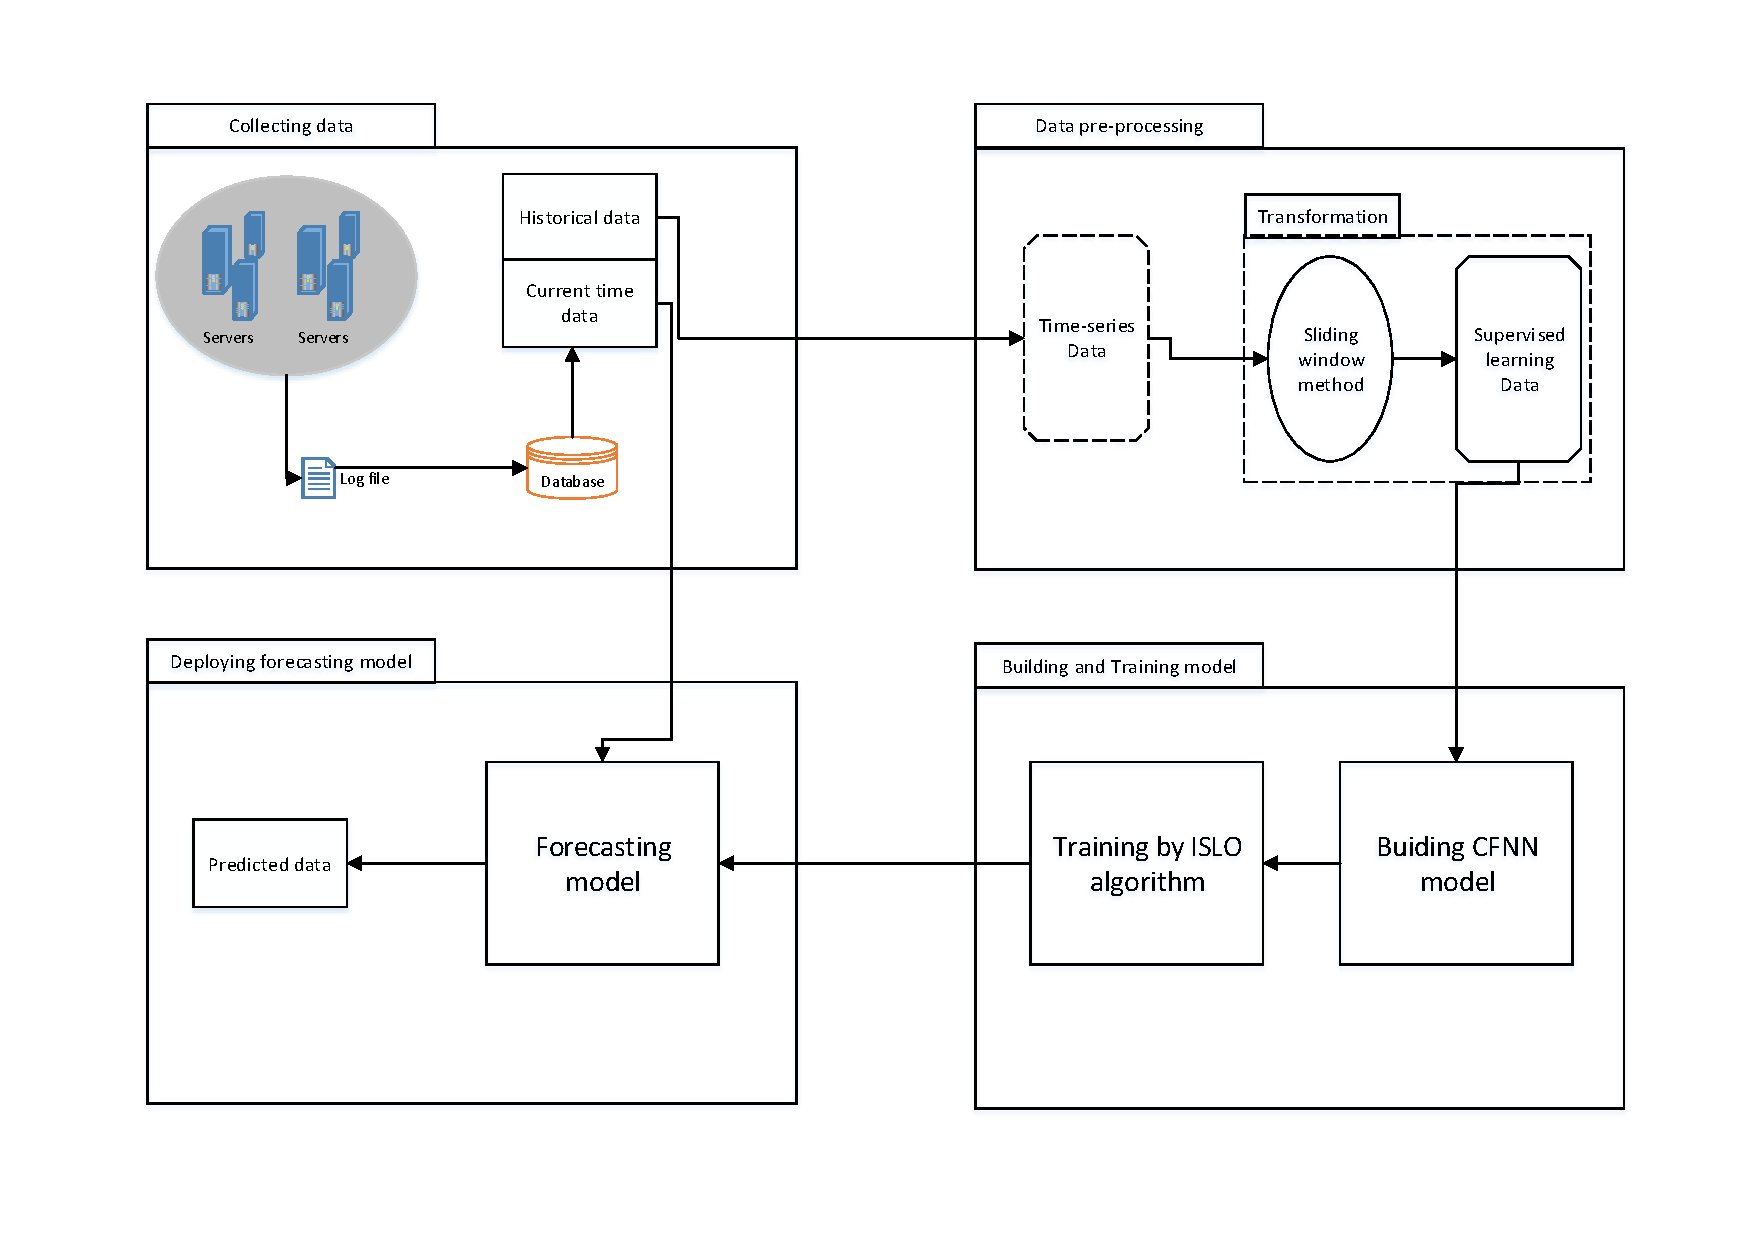
\includegraphics[width=1.0\linewidth]{/pdf/model/model_phases}
  \caption{Proposed model design} 
  \label{fig_model_phases} 
\end{figure}
	
\subsection{Collecting data}
\label{collect_data}
	
	Before building any forecasting systems, the very first and the most important task that must be done is collecting data. Therefore, we collect data recording the resource usage of Google (Google Cluster Trace data) and Internet Traffic data collected from a private internet service provider (ISP) in Europe and the United Kingdom (these datasets  will be discuss in detail in Chapter \ref{ch:experiments}. The data collected contains two main parts: the data from history that we use for training, and current time data that we use for predicting resource usage in the future.  
	

\subsection{Data pre-processing}
\label{data-pre}

\begin{table}[!t]
\caption{Time-series data and Supervised learning data comparison}
\label{tbl_data_cmp}
\centering
\begin{tabular}{|p{6cm}|p{6cm}|}
 \hline
 Time-series data & Supervised Learning data  \\ 
 \hline
 1. Time 1, value 1 & 1. Input 1, output 1  \\ 
 2. Time 2, value 2 & 2. Input 2, output 2  \\ 
 3. Time 3, value 3 & 3. Input 3, output 3  \\ 
 \hline
\end{tabular}
\end{table}
	
	This phase play a role as a pre-processor transforming the raw data into the kind of data that can be used in neural networks. In order to learn, models need both training data and testing data. We create the data for models through several steps as follows:

\begin{itemize}
\item  Evaluate and choose carefully which columns of data are needed for the forecasting model.
\item  The parts of data chosen are then normalized in the range $[ \, 0, 1 ] \,$.
\item Transform time-series data into supervised learning data using \textit{Sliding window} technique.
\item Divide processed data into two sets: training set and testing set.
\end{itemize}

	The step $3th$ of the pre-processing phase is necessary because time-series data is the data recorded through time, and there is no term of features and output data. Therefore, we need to transform this data into supervised learning data, that contains input features, and output. Table \ref{tbl_data_cmp} depicts the difference between time-series data and normal data used in supervised learning.


	In order to create data for supervised learning, we use the method called \textit{Sliding window}. This method takes the data of $k$ values before the time $t$ as the features and output data is the value at the time $t$. For example, when $k=3$, the results of data transformation is shown as in Table \ref{tbl_sliding_window}.
	
\begin{table}[!t]
\caption{Example of data transformation using Sliding window method}
\label{tbl_sliding_window}
\centering
\begin{tabular}{|p{4cm}|p{2cm}|p{2cm}|p{2cm}|p{2cm}|}
 \hline
 \multicolumn{1}{|c|}{Time-series data} & \multicolumn{4}{c|}{Transformed data} \\ 
 \hline
 \multicolumn{1}{|c}{} & \multicolumn{3}{|c}{Input} & \multicolumn{1}{|c|}{Output} \\
 \hline
  Time $(t=4)$, Value 4 & Value 1 & Value 2 & Value 3 & Value 4 \\
  Time $(t=5)$, Value 5 & Value 2 & Value 3 & Value 4 & Value 5 \\
  Time $(t=6)$, Value 6 & Value 3 & Value 4 & Value 5 & Value 6 \\
  Time $(t=7)$, Value 7 & Value 4 & Value 5 & Value 6 & Value 7 \\
 ... & ... & ... & ...  & ... \\
 \hline
\end{tabular}
\end{table}	
	 
\subsection{Building and Training model}
\label{main_model}

	In this phase, pre-processed data is used for training our proposed model called ISLO-CFNN, which is CFNN being trained by the optimization of ISLO algorithm. ISLO algorithm is applied to train a CFNN model with one hidden layer. There is two key aspects needed to be taken into consideration: firstly, the formation of an agent in ISLO and the selection of fitness function.
	
	Firstly, each agent in the population in ISLO are presented as one solution for CFNN model, which means that a search agent is a one-dimensional vector created by concatenating weights and biases of CFNN. Therefore, the features of a search agent contains three elements: a set of weights connecting the input layer with hidden layer, a set of weights connecting the hidden layer with output layer and also and a set of weights connecting the input layer with output layer. Therefore,  the length of a solution can be calculated by Eq. \ref{eq_length_solution}.	
\begin{equation} \label{eq_length_solution}
	Solution\_length = (1+i)*h + (1+h)*o + (1+i)*o
\end{equation}
Where $i, h, o$ is the number of input, hidden and output neurons,  respectively (in time-series prediction, the number of output neurons is one).
\begin{figure}[!ht] 
   \centering
   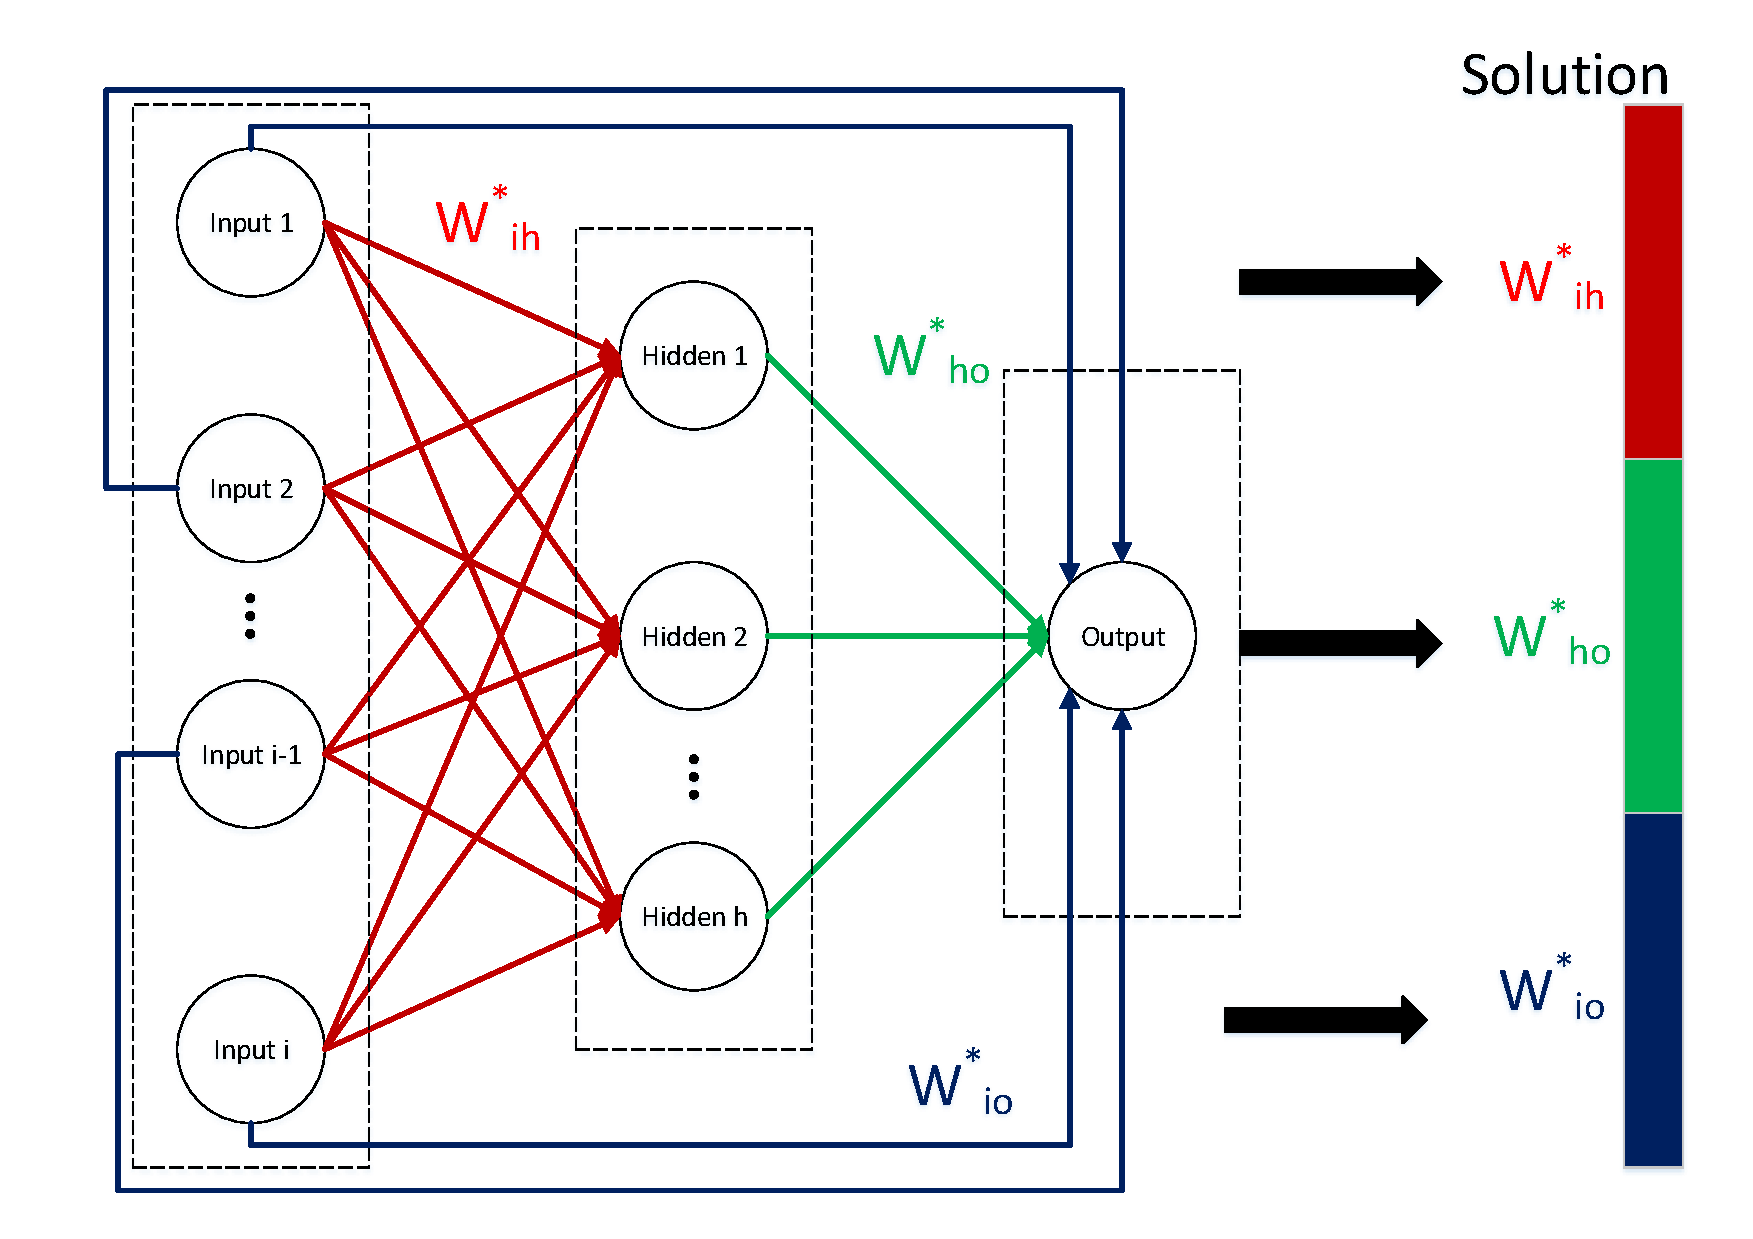
\includegraphics[width=0.75\linewidth]{pdf/model/solution_creation}
  \caption{Encoding process transforming a parameter set in CFNN into an agent in ISLO algorithm. ($W^*$ indicates weights and biases between 2 layers)} 
  \label{fig_solution_encode} 
\end{figure}
	
	Secondly, the fitness value of each agent in ISLO is considered as the loss value of the CFNN model with the parameter set from the agent and input data. We utilize the loss function Mean Square Error (MSE) to calculate the difference between the actual and predicted output values by generated agent for all samples in the training set. 
\begin{figure}[!ht] 
   \centering
   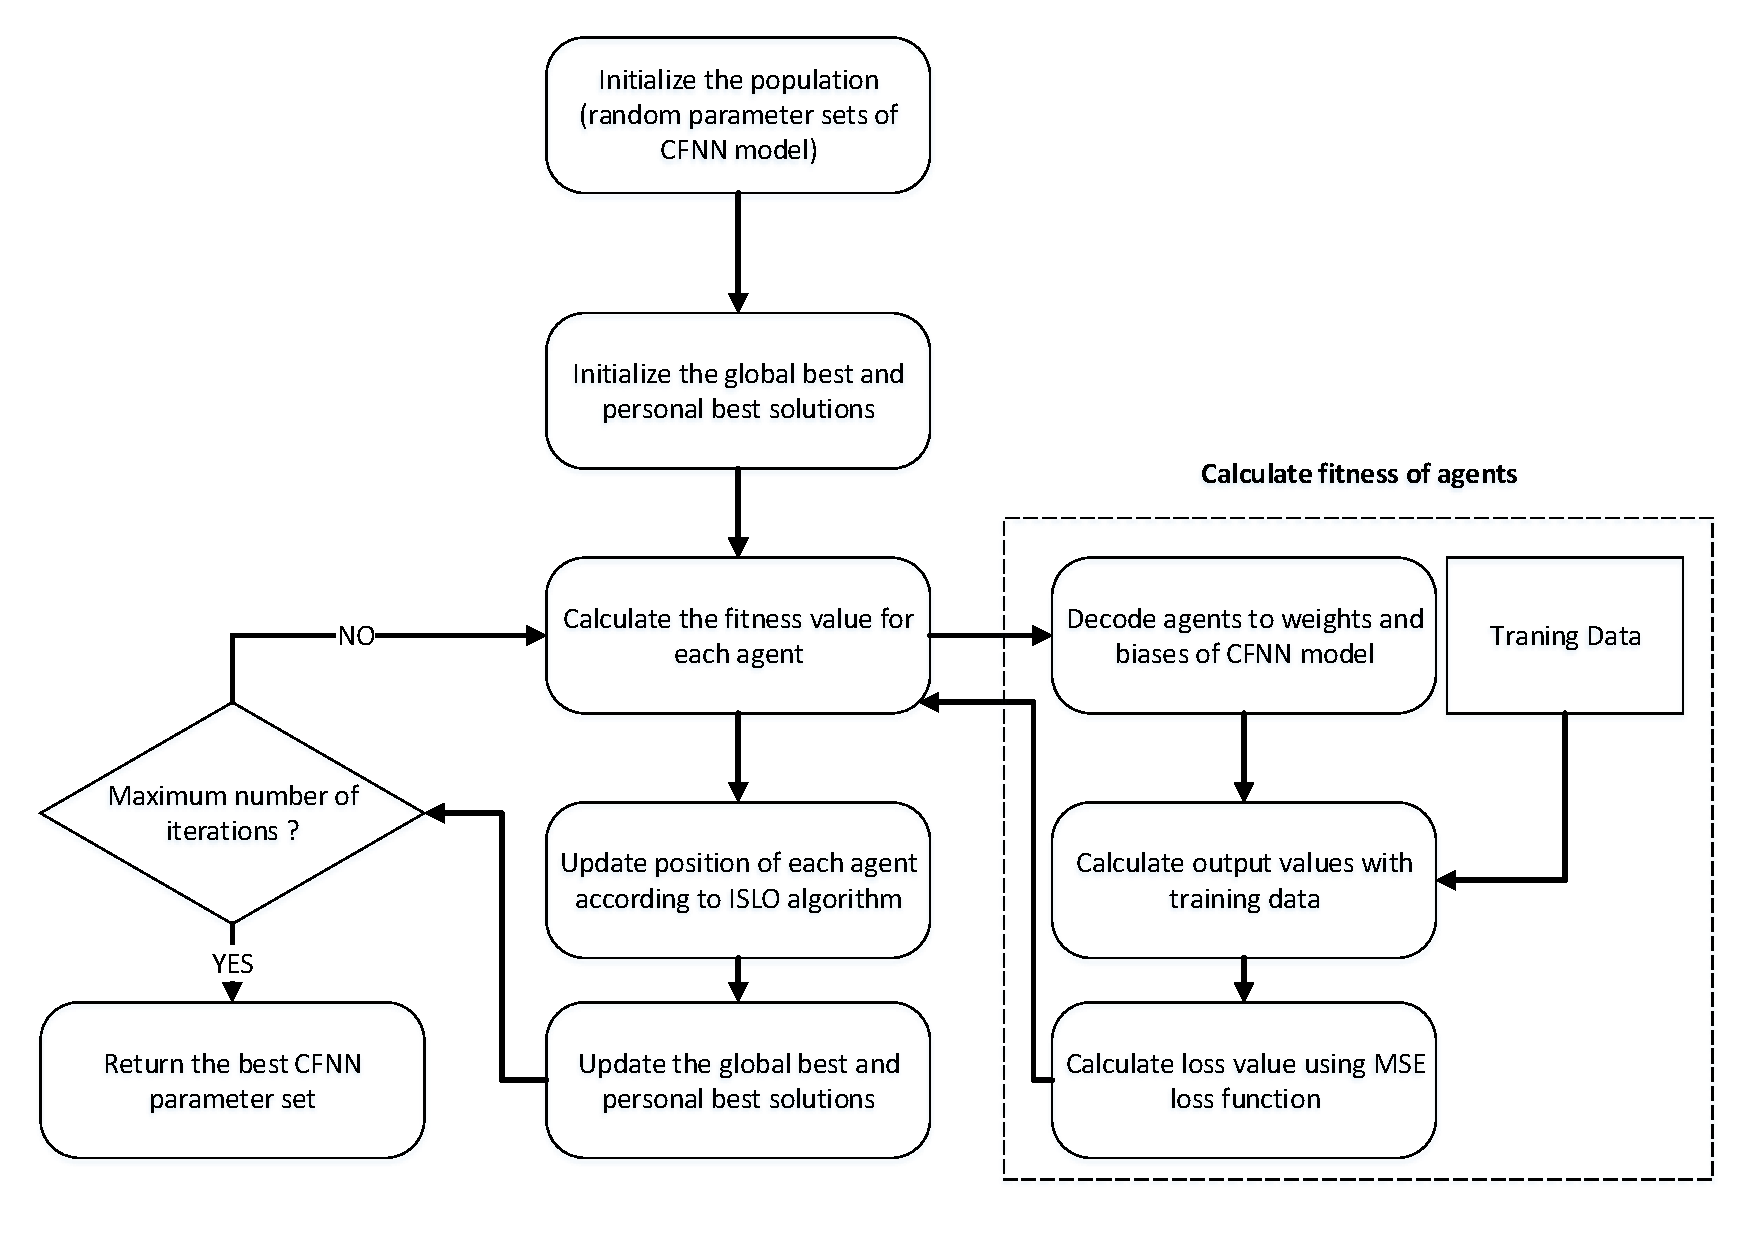
\includegraphics[width=1.0\linewidth]{pdf/model/islo_cfnn_workflow}
  \caption{The work flow of ISLO-CFNN model.} 
  \label{fig_islo_cfnn_workflow} 
\end{figure}	

	The workflow of ISLO applied in this work for training CFNN are depicted in Fig. \ref{fig_islo_cfnn_workflow}, and can be generally presented by the following steps:
	
\begin{enumerate}
\item Initialization: pre-define the number of search agents in ISLO, which are randomly generated in the range [-1, 1]. Each parameter set of CFNN model is encoded to a vector playing a role as an agent in ISLO population. (See in Fig. \ref{fig_solution_encode})
\item Calculate fitness value for each search agent: The quality of a solution is measured by the loss value of CFNN output. After being decoded into weights and biases vectors, a solution will be applied to form a CFNN model. Data samples in training set is then feed-forwarded through the network, generating predicted output values. Finally, the fitness value is calculated as the difference between predicted and actual output values through the MSE loss function.
\item Update positions of all search agents following formulas of ISLO algorithm.
\item Steps 2 and 3 are repeated until the difference is close enough, or the maximum number of iterations is reached.
\item Return the best CFNN parameter set. 
\end{enumerate}
	     
\subsection{Deploy prediction model}
\label{deploy}
	
	After obtaining CFNN model with the best parameter set by ISLO algorithm, the model is installed on servers and ready to predict the demand for resources in the future based on historical data.   
	  
\chapter{Experiments}
\label{ch:experiments}
The optimization capacity of ISLO algorithm developed in this study would be tested by solving two experiments: one for theoretical test and another for an optimizing application in the real world.
 
	In the theoretical test, 30 benchmark functions are used for testing the numerical efficiency of ISLO. The set of benchmark functions cover a wide range function groups including: classical unimodal and multimodal functions, hybrid functions and composition functions which are considered in CEC 2014 and CEC 2015 special session (See \cite{liang2013problem} and \cite{liang2014problem} for more information about the annual competition). ISLO will be compared with several well-known algorithms in all four groups in meta-heuristic optimization algorithms including evolutionary, swarm-based, physical-based and human-based algorithms.
	
	On the other hand, the optimizing performance of ISLO is also tested in a time-series prediction problem. Specifically, the proposed model in \ref{sec:proposed_model} is used for the experiment with three real-world datasets, which are Google Trace data, EU Internet Traffic data and UK Internet Traffic data in different perspectives. The results are compared with that of several deep learning models that are widely used for time-series prediction, and additionally, the performance of ISLO in optimizing CFNN is also compared with several algorithms in the first experiment. 
	
	The detail of each experiment as well as results and analysis are presented as below.
	
\section{Theoretical experiments}
\label{sec:exp_theory}

	The performance of ISLO is theoretically experimented by 30 benchmark functions. They are divided into four groups of functions:
\begin{itemize}
\item Unimodal benchmark functions: they have only one global optimal point in the search space.
\item Multimodal benchmark functions: they have one global optimal point going along with local minimum points.
\item Hybrid functions:  the variables are
randomly divided into some sub-components and then different basic unimodal and multimodal functions are used for different sub-components.
\item Composition functions: they merge the properties of the sub-functions better and maintains continuity around the global/local optima. 
\end{itemize}

\begin{figure}[!ht] 
   \centering
   \begin{subfigure}{0.24\textwidth}
   	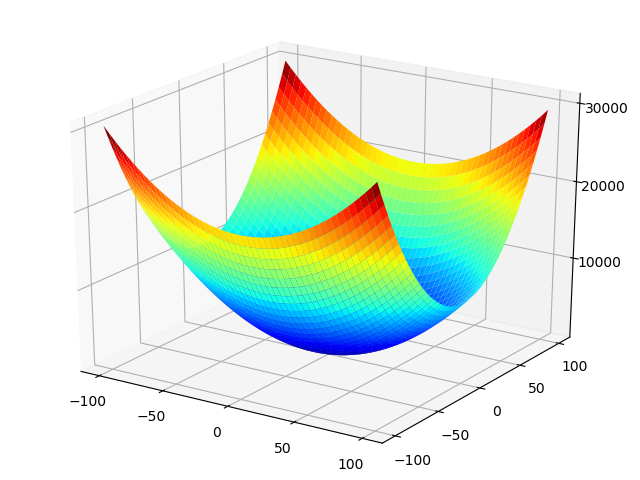
\includegraphics[width=1\linewidth]{png/functions/uni_f5}
  	 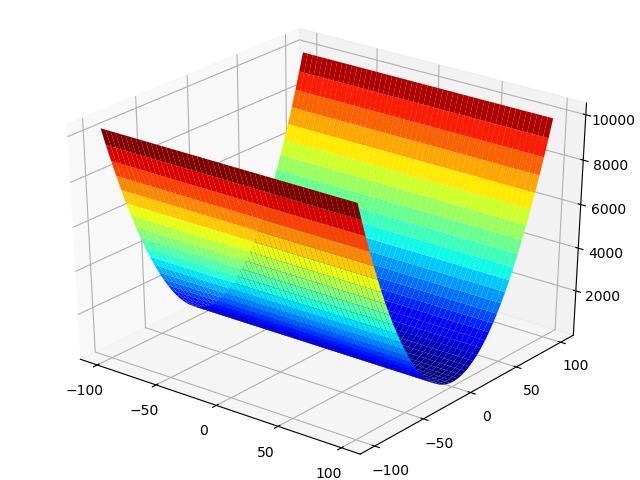
\includegraphics[width=1\linewidth]{png/functions/uni_f7}
  	\caption{Unimodal}
  	\label{subfig:uni}
  	\end{subfigure}
    \begin{subfigure}{0.24\textwidth}
   	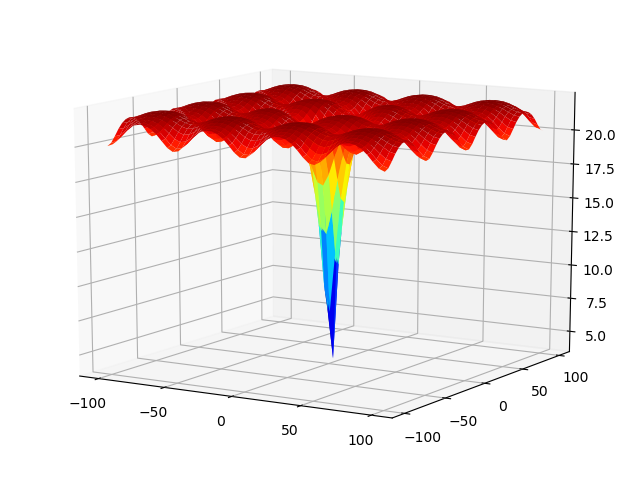
\includegraphics[width=1\linewidth]{png/functions/multi_f9}
  	 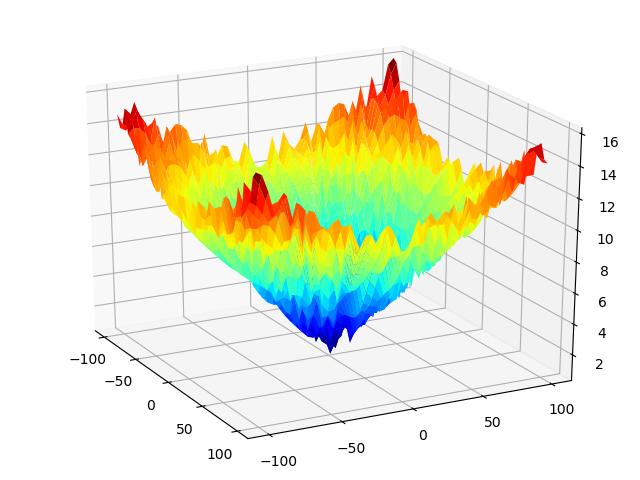
\includegraphics[width=1\linewidth]{png/functions/multi_f12}
  	 \caption{Multimodal}
  	\label{subfig:multi}
  	\end{subfigure}
   \begin{subfigure}{0.24\textwidth}
   	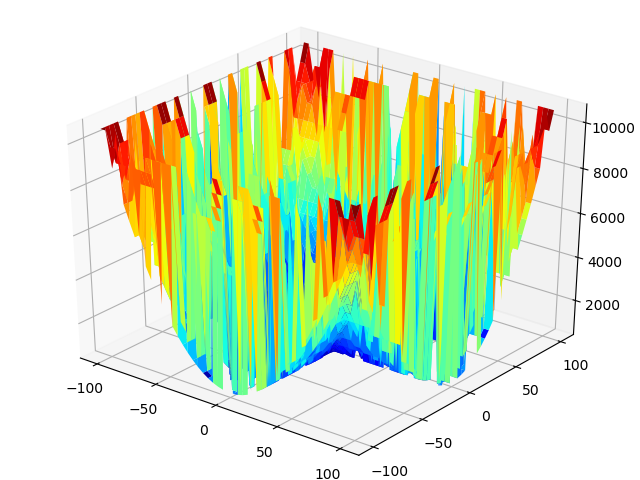
\includegraphics[width=1\linewidth]{png/functions/hybrid_f21}
  	 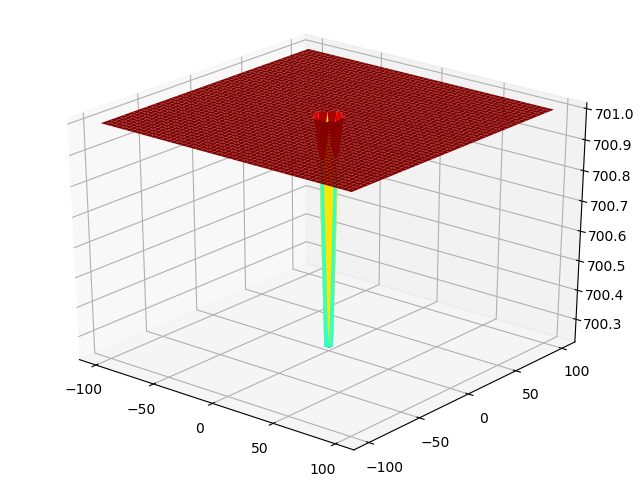
\includegraphics[width=1\linewidth]{png/functions/hybrid_f22}
  	 \caption{Hybrid}
  	\label{subfig:hybrid}
  	\end{subfigure}
  	\begin{subfigure}{0.24\textwidth}
   	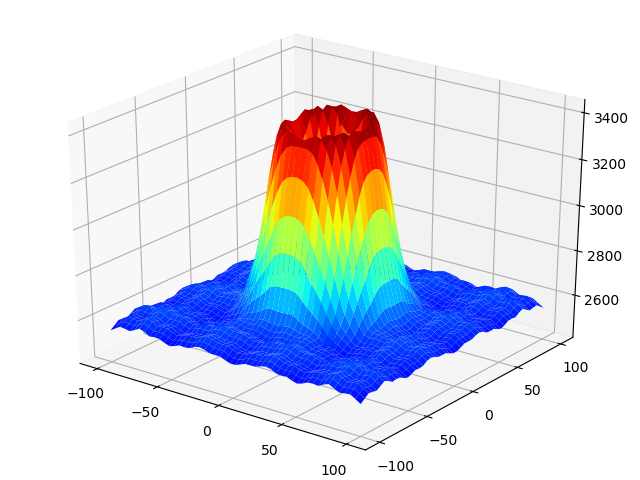
\includegraphics[width=1\linewidth]{png/functions/compos_f26}
  	 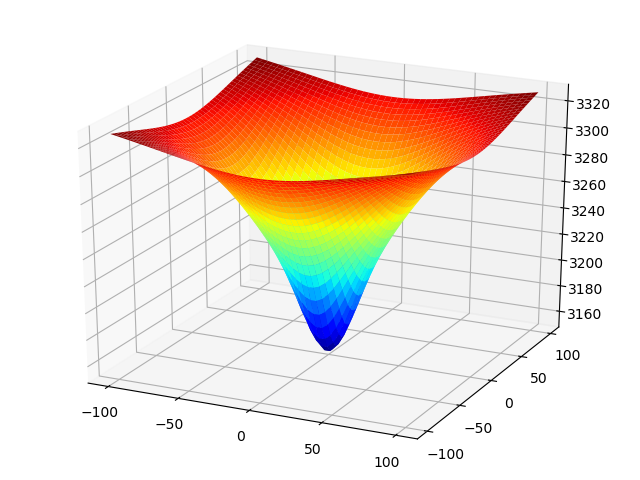
\includegraphics[width=1\linewidth]{png/functions/compos_f30}
  	 \caption{Composition}
  	\label{subfig:compos}
  	\end{subfigure}
  \caption{Examples of 3D plot for each kind of benchmark functions.} 
  \label{fig_functions} 
\end{figure}

The detail such as name, formula, search space and optimal value of each function is shown in Table. [\ref{tbl_uni_funcs}-\ref{tbl_compos_funcs}]. Also, Fig. \ref{fig_functions} presents the typical 3D plots of the cost function for some test cases considered in this study. 

\begin{table}[!t]
\caption{Description of unimodal benchmark functions}
\label{tbl_uni_funcs}
\centering
\begin{tabular}{p{9cm} p{2cm} p{1cm}}
 \hline Mathematical Definition & Range & $f_{min}$  \\ 
 \hline
$f_1(x) = \sum_{i=1}^n x_i^2$ & [-500, 500] & 0 \\
$f_2(x) =  \sum_{i=1}^n |x_i|$ & [-500, 500] & 0 \\
$f_3(x) =  max_{i = 1, 2,...,n}|x_i|)$ & [-500, 500] & 0 \\
$f_4(x) =  \sum_{i=1}^n |x_i| + \prod_{i=1}^n |x_i|$  & [-500, 500] & 0 \\
$f_5(x) =  \sum_{i=1}^n ix_i^2$ & [-500, 500] & 0 \\
$f_6(x) =  \sum_{i=1}^{n-1} (x_i^2)^{x_{i+1}^2+1} + (x_{i+1}^2)^{x_{i}^2+1}$ & [-500, 500] & 0 \\
$f_7(x) =  \sum_{i=1}^n (10^6)^{\frac{x_i-1}{n-1}} + 100$ & [-500, 500] & 100 \\
$f_8(x) = x_1^2 + 10^6\sum_{i=2}^n x_i^2$ + 200 & [-500, 500] & 200 \\
 \hline
\end{tabular}
\end{table}

\begin{table}[!t]
\caption{Description of multimodal benchmark functions}
\label{tbl_multi_funcs}
\centering
\begin{tabular}{p{9cm} p{2cm} p{1cm}}
 \hline 
 Mathematical Definition & Range & $f_{min}$  \\ 
 \hline
$f_9(x) = -a.exp(-b\sqrt{\frac{1}{n}\sum_{i=1}^{n}x_i^2})-exp(\frac{1}{n}\sum_{i=1}^{n}cos(cx_i))+ a + exp(1)$ with a = 20 and b = 0.2 & [-500, 500] & 0 \\
$f_{10}(x) =\left[\left(||\textbf{x}||^2 - n\right)^2\right]^\alpha + \frac{1}{n}\left(\frac{1}{2}||\textbf{x}||^2+\sum_{i=1}^{n}x_i\right)+\frac{1}{2}$ & [-500, 500] & 0 \\
$f_{11}(x) =\sum_{i=1}^{n}(x^2-i)^2$ & [-500, 500] & 0 \\
$f_{12}(x)=1-cos(2\pi\sqrt{\sum_{i=1}^{D}x_i^2})+0.1\sqrt{\sum_{i=1}^{D}x_i^2}$ & [-500, 500] & 0 \\
$f_{13}f(x)=\sum_{i=1}^{n}[b (x_{i+1} - x_i^2)^ 2 + (a - x_i)^2]$ & [-500, 500] & 0 \\
$f_{14}(x) = \sum_{i=1}^{n}{\sum_{j=1}^5{j sin((j+1)x_i+j)} + 300}$ & [-500, 500] & 300 \\
$f_{15}(x)=10n + \sum_{i=1}^{n}(x_i^2 - 10cos(2\pi x_i)) + 400$ & [-500, 500] & 400 \\
$f_{16}(x) = 418.9829D -{\sum_{i=1}^{n} x_i sin(\sqrt{|x_i|})}. + 500$ & [-500, 500] & 500 \\
\hline
\end{tabular}
\end{table}

The performance of ISLO algorithm about optimizing 30 benchmark functions is compared with different optimizers including well-known algorithms as well as recent algorithms that belong to all four groups in nature-inspired meta-heuristic algorithms. Specifically, they are: 
\begin{itemize}
\item Generic Algorithm (GA) \cite{whitley1994genetic} (Evolutionary algorithms)
\item Particle Swarm Optimization (PSO) \cite{kennedy2010particle}, Whale Optimization Algorithm (WOA) \cite{mirjalili2016whale} and the original Sea Lion Optimization Algorithm (SLnO) \cite{masadeh2019sea} (Swarm-based algorithms)
\item Tug of War Optimization (TWO) \cite{kaveh2016novel} (Physics-based algorithms)
\item Queuing Search Optimization (QSO) \cite{zhang2018queuing} (Human-based algorithms)
\end{itemize}

\begin{table}[!t]
\caption{Description of hybrid benchmark functions}
\label{tbl_hybrid_funcs}
\centering
\begin{tabular}{p{9cm} p{2cm} p{1cm}}
 \hline Mathematical Definition & Range & $f_{min}$  \\ 
 \hline
$f_{17}$ (function 17 in CEC 2014) & \multirow{3}{*}{[-500, 500]} & \multirow{3}{*}{1700} \\
p = [0.3, 0.4, 0.3] & \\
Modified Schwefel's , Rastrigin's  and High Conditioned Elliptic Functions & \\ \hline
$f_{18}$ (function 18 in CEC 2014) & \multirow{3}{2cm}{[-500, 500]} & \multirow{3}{1cm}{1800} \\
p = [0.3, 0.4, 0.3] & \\
Bent Cigar, HGBat and Rastrigin’s Functions & \\ \hline
$f_{19}$ (function 19 in CEC 2014) & \multirow{3}{2cm}{[-500, 500]} & \multirow{3}{1cm}{1900} \\
p = [ 0.2, 0.2, 0.3, 0.3] & \\
Griewank’s, Weierstrass, Rosenbrock’s and Scaffer’s Functions & \\ \hline
$f_{20}$ (function 20 in CEC 2014) & \multirow{3}{2cm}{[-500, 500]} & \multirow{3}{1cm}{2000} \\
p =  [0.2, 0.2, 0.3, 0.3] & \\
HGBat , Discus, Expanded Griewank’s plus Rosenbrock’s  and Rastrigin’s Functions & \\ \hline
$f_{21}$ (function 6 in CEC 2015) & \multirow{3}{2cm}{[-500, 500]} & \multirow{3}{1cm}{600} \\
p =  [0.3,0.3,0.4]  & \\
Modified Schwefel's , Rastrigin's, High Conditioned Elliptic Functions & \\ \hline
$f_{22}$ (function 7 in CEC 2015) & \multirow{3}{2cm}{[-500, 500]} & \multirow{3}{1cm}{700} \\
p =[0.2,0.2,0.3,0.3]  & \\
Griewank's , Weierstrass ,Rosenbrock's and Scaffer's Functions & \\ \hline
$f_{23}$ (function 8 in CEC 2015) & \multirow{3}{2cm}{[-500, 500]} & \multirow{3}{1cm}{800} \\
p = [0.1,0.2,0.2,0.2,0.3]  & \\
Scaffer’s , HGBat ,Rosenbrock’s, Modified Schwefel’s and High Conditioned Elliptic Functions & \\ \hline
\end{tabular}
\end{table}

\begin{table}[!t]
\caption{Description of composition benchmark functions}
\label{tbl_compos_funcs}
\centering
\begin{tabular}{p{9cm} p{2cm} p{1cm}}
 \hline Mathematical Definition & Range & $f_{min}$  \\ 
 \hline
$f_{24}$ (function 9 in CEC 2015) & \multirow{4}{*}{[-500, 500]} & \multirow{3}{*}{900} \\
$\sigma = $ [20, 20, 20] & \\
$\lambda = $ [1, 1, 1] & \\
Schwefel's , Rastrigin's  and  HGBat  Functions & \\ \hline
$f_{25}$ (function 10 in CEC 2015) & \multirow{4}{*}{[-500, 500]} & \multirow{3}{*}{1000} \\
$\sigma = $  [10, 30,50]  & \\
$\lambda = $  [1, 1, 1]  & \\
$f_{21}$, $f_{22}$ and $f_{23}$ Functions & \\ \hline
$f_{26}$ (function 11 in CEC 2015) & \multirow{4}{*}{[-500, 500]} & \multirow{3}{*}{1100} \\
$\sigma = $  [10, 10, 10, 20, 20]  & \\
$\lambda = $  [10, 10, 2.5, 25,1e-6]  & \\
 HGBat ,  Rastrigin’s  and   Schwefel's,  Weierstrass and  High Conditioned Elliptic   Functions & \\ \hline
$f_{27}$ (function 12 in CEC 2015) & \multirow{4}{*}{[-500, 500]} & \multirow{3}{*}{1200} \\
$\sigma = $  [10,20,20,30,30] & \\
$\lambda = $ [0.25, 1, 1e-7, 10, 10]  & \\
 Schwefel's  , Rastrigin's  and   High Conditioned Elliptic, Expanded Scaffer’s and  HappyCat Functions & \\ \hline
$f_{28}$ (function 13 in CEC 2015) & \multirow{4}{*}{[-500, 500]} & \multirow{3}{*}{1300} \\
$\sigma = $  [10, 10, 10, 20, 20]  & \\
$\lambda = $  [1, 10, 1, 25, 10]  & \\
$f_{23}$ , Rastrigin's  and  $f_{21}$,  Schwefel's  and  Expanded Scaffer’s  Functions & \\ \hline
$f_{29}$ (function 14 in CEC 2015) & \multirow{4}{*}{[-500, 500]} & \multirow{3}{*}{1400} \\
$\sigma = $  [10, 20, 30, 40, 50, 50, 50] & \\
$\lambda = $  [10,2.5, 2.5, 10,1e-6,1e-6, 10] & \\
HappyCat , Griewank’s plus Rosenbrock’s, Schwefel's, Expanded Scaffer’s, High Conditioned Elliptic, Cigar and  and Rastrigin’s  Functions & \\ \hline
$f_{30}$ (function 15 in CEC 2015) & \multirow{4}{*}{[-500, 500]} & \multirow{3}{*}{1500} \\
$\sigma = $  [10, 10, 20, 20, 30, 30, 40, 40, 50, 50] & \\
$\lambda = $  [0.1,2.5e-1, 0.1, 2.5e-2, 1e-3, 0.1, 1e-5, 10, 2.5e-2, 1e-3] & \\
Rastrigin’s  , Weierstrass, HappyCat, Schwefel's, Rosenbrock's, HGBat, Katsuura, Expanded Scaffer’s, Expanded Griewank’s  and  Ackley  Functions & \\ \hline

\end{tabular}
\end{table}

\subsection{Evaluation method and Parameter settings}

	With compared algorithms and functions mentioned above, the experimental results of each model are produced by calculating mean and standard deviation ($std$) value (Eq. \ref{eq_mean} and \ref{eq_std}) of 20 times running starting from randomly generated populations for each algorithms. For all the algorithms, a population size and maximum iteration equal to 100 and 500 have been utilized to run on each function with 50-dimension search space. The choices  of parameters are based on existing setting up
described in original paper of each algorithm.
\begin{equation} \label{eq_mean}
mean = \frac{1}{n}\sum_{i=1}^n r_i
\end{equation}
\begin{equation}\label{eq_std}
std = \sqrt{\frac{1}{n-1}\sum_{i=1}^n(r_i - r)^2}
\end{equation}
where $N$ is the number of values and $r_i$ $(i = 1, 2, ..., N)$ are observations.
	
	For each function, after calculating $mean$ and $std$ values of each algorithm, the best results will be highlighted in both. The best results are determined by following rules:
\begin{itemize}
\item $mean$ values are considered at first. If in a case, an algorithm own the best $mean$ value, it will be ranked as the best optimizer.
\item In the case where there are two or more algorithms having the same $mean$ value, the one that has the most stable $std$ value will be chosen as the best one.
\end{itemize}
	
	Finally, the experimental results of all functions and algorithms are shown in Table \ref{tbl_results_uni_multi} and \ref{tbl_results_hybrid_compos}, and the convergence speeds of the algorithms in several functions are illustrated in Fig. \ref{fig_uni_multi_convergence} and \ref{fig_hybrid_compos_convergence}.

\begin{table}[!t]
\caption{Comparison of optimization results obtained for the unimodal and multimodal functions}
\label{tbl_results_uni_multi}
\centering
\resizebox{\textwidth}{!}{%
\begin{tabular}{|l|l|l|l|l|l|l|l|l|}
\hline
Function             &      & GA       & PSO      & SLnO     & WOA               & ISLO               & TWO      & QSO               \\ \hline
\multirow{3}{*}{$f_1$}  & mean & 4.64E+01 & 9.69E+02 & 2.52E-25 & 2.26E-80          & \textbf{3.26E-120} & 1.06E+01 & 8.14E-01          \\ \cline{2-9} 
                     & std  & 7.54E+00 & 3.12E+02 & 7.11E-25 & 9.41E-80          & \textbf{8.45E-120} & 1.39E+00 & 3.08E-01          \\ \cline{2-9} 
                     & rank & 6        & 7        & 3        & 2                 & \textbf{1}         & 5        & 4                 \\ \hline
\multirow{3}{*}{$f_2$}  & mean & 2.19E+02 & 1.99E+02 & 1.64E+01 & 2.98E+00          & \textbf{2.26E-01}  & 2.49E+01 & 2.62E+00          \\ \cline{2-9} 
                     & std  & 1.44E+01 & 3.42E+01 & 2.38E+00 & 5.86E-01          & \textbf{1.23E-01}  & 2.24E+00 & 6.15E-01          \\ \cline{2-9} 
                     & rank & 7        & 6        & 4        & 3                 & \textbf{1}         & 5        & 2                 \\ \hline
\multirow{3}{*}{$f_3$}  & mean & 4.30E+00 & 1.79E+01 & 7.58E+01 & 4.39E+01          & \textbf{6.25E-58}  & 1.58E+01 & 1.82E+01          \\ \cline{2-9} 
                     & std  & 1.11E+00 & 2.28E+00 & 1.92E+01 & 2.29E+01          & \textbf{2.64E-57}  & 3.93E+00 & 1.43E+00          \\ \cline{2-9} 
                     & rank & 2        & 4        & 7        & 6                 & \textbf{1}         & 3        & 5                 \\ \hline
\multirow{3}{*}{$f_4$}  & mean & 1.12E+02 & 7.43E+02 & 4.07E+26 & 2.81E+00          & \textbf{1.56E-01}  & 1.71E+32 & 1.79E+02          \\ \cline{2-9} 
                     & std  & 7.57E+00 & 1.22E+02 & 1.30E+27 & 7.00E-01          & \textbf{1.01E-01}  & 7.33E+32 & 1.98E+02          \\ \cline{2-9} 
                     & rank & 3        & 5        & 6        & 2                 & \textbf{1}         & 7        & 4                 \\ \hline
\multirow{3}{*}{$f_5$}  & mean & 1.36E+03 & 1.58E+04 & 2.01E+02 & 2.42E+00          & \textbf{3.52E-02}  & 2.24E+03 & 2.43E+01          \\ \cline{2-9} 
                     & std  & 3.87E+02 & 5.57E+03 & 9.51E+01 & 6.70E-01          & \textbf{6.06E-02}  & 1.06E+03 & 1.20E+01          \\ \cline{2-9} 
                     & rank & 5        & 7        & 4        & 2                 & \textbf{1}         & 6        & 3                 \\ \hline
\multirow{3}{*}{$f_6$}  & mean & 1.27E+00 & 1.20E+00 & 3.27E-01 & 4.71E-03          & \textbf{5.65E-05}  & 1.02E+00 & 7.83E-02          \\ \cline{2-9} 
                     & std  & 3.01E-02 & 4.08E-02 & 1.47E-01 & 1.40E-03          & \textbf{5.50E-05}  & 2.21E-02 & 4.22E-02          \\ \cline{2-9} 
                     & rank & 7        & 6        & 4        & 2                 & \textbf{1}         & 5        & 3                 \\ \hline
\multirow{3}{*}{$f_7$}  & mean & 8.70E+06 & 2.34E+07 & 1.42E+06 & 6.12E+04          & \textbf{8.22E+02}  & 1.22E+08 & 1.27E+04          \\ \cline{2-9} 
                     & std  & 2.66E+06 & 1.17E+07 & 1.12E+06 & 2.05E+04          & \textbf{1.10E+02}  & 4.97E+07 & 5.12E+03          \\ \cline{2-9} 
                     & rank & 5        & 6        & 4        & 3                 & \textbf{1}         & 7        & 2                 \\ \hline
\multirow{3}{*}{$f_8$}  & mean & 4.54E+08 & 7.70E+09 & 6.52E+07 & 7.83E+05          & \textbf{1.60E+04}  & 1.02E+08 & 8.19E+06          \\ \cline{2-9} 
                     & std  & 1.10E+08 & 2.70E+09 & 2.65E+07 & 2.47E+05          & \textbf{1.20E+04}  & 1.42E+07 & 3.40E+06          \\ \cline{2-9} 
                     & rank & 6        & 7        & 4        & 2                 & \textbf{1}         & 5        & 3                 \\ \hline
                     \multirow{3}{*}{$f_9$}  & mean & 1.69E+01 & 2.04E+01 & 2.05E+01 & 2.82E-01          & \textbf{1.85E-02}  & 2.01E+01 & 2.08E+01          \\ \cline{2-9} 
                     & std  & 3.02E-01 & 8.70E-01 & 3.00E-01 & 2.22E-01          & \textbf{1.11E-02}  & 3.89E-02 & 2.81E-02          \\ \cline{2-9} 
                     & rank & 3        & 5        & 6        & 2                 & \textbf{1}         & 4        & 7                 \\ \hline
\multirow{3}{*}{$f_{10}$} & mean & 6.71E+00 & 1.42E+01 & 3.55E-01 & 3.41E-01          & \textbf{4.34E-04}  & 7.68E-01 & 7.05E-01          \\ \cline{2-9} 
                     & std  & 9.85E-01 & 3.00E+00 & 8.31E-02 & 1.35E-01          & \textbf{1.89E-03}  & 1.25E-01 & 6.88E-02          \\ \cline{2-9} 
                     & rank & 6        & 7        & 3        & 2                 & \textbf{1}         & 5        & 4                 \\ \hline
\multirow{3}{*}{$f_{11}$} & mean & 2.11E+04 & 2.99E+04 & 5.25E+03 & \textbf{3.14E+03} & 9.01E+03           & 5.20E+03 & 6.09E+03          \\ \cline{2-9} 
                     & std  & 2.43E+03 & 1.50E+04 & 3.25E+03 & \textbf{1.42E+03} & 5.01E+02           & 1.77E+03 & 7.24E+02          \\ \cline{2-9} 
                     & rank & 6        & 7        & 3        & \textbf{1}        & 5                  & 2        & 4                 \\ \hline
\multirow{3}{*}{$f_{12}$} & mean & 3.84E+00 & 5.30E+00 & 7.25E-01 & 3.75E-01          & \textbf{9.50E-02}  & 1.76E+00 & 1.87E+00          \\ \cline{2-9} 
                     & std  & 3.09E-01 & 5.25E-01 & 6.98E-02 & 9.94E-02          & \textbf{2.00E-02}  & 3.93E-01 & 2.05E-01          \\ \cline{2-9} 
                     & rank & 6        & 7        & 3        & 2                 & \textbf{1}         & 4        & 5                 \\ \hline
\multirow{3}{*}{$f_{13}$} & mean & 8.18E+04 & 4.77E+06 & 1.45E+03 & 5.63E+01          & \textbf{3.85E-01}  & 5.40E+04 & 6.70E+03          \\ \cline{2-9} 
                     & std  & 1.97E+04 & 2.83E+06 & 5.67E+02 & 2.75E+00          & \textbf{3.67E-01}  & 9.53E+04 & 4.26E+03          \\ \cline{2-9} 
                     & rank & 6        & 7        & 3        & 2                 & \textbf{1}         & 5        & 4                 \\ \hline
\multirow{3}{*}{$f_{14}$} & mean & 3.17E+02 & 3.20E+02 & 3.21E+02 & 3.00E+02          & \textbf{3.00E+02}  & 3.20E+02 & 3.21E+02          \\ \cline{2-9} 
                     & std  & 3.42E-01 & 7.51E-01 & 2.93E-01 & 1.92E-01          & \textbf{1.37E-02}  & 3.78E-02 & 2.91E-02          \\ \cline{2-9} 
                     & rank & 3        & 5        & 7        & 2                 & \textbf{1}         & 4        & 6                 \\ \hline
\multirow{3}{*}{$f_{15}$} & mean & 2.75E+04 & 7.21E+04 & 4.21E+03 & 5.42E+02          & \textbf{4.02E+02}  & 3.17E+05 & 4.46E+02          \\ \cline{2-9} 
                     & std  & 9.46E+03 & 3.66E+04 & 2.29E+03 & 5.50E+01          & \textbf{2.43E+00}  & 1.28E+05 & 3.07E+01          \\ \cline{2-9} 
                     & rank & 5        & 6        & 4        & 3                 & \textbf{1}         & 7        & 2                 \\ \hline
\multirow{3}{*}{$f_{16}$} & mean & 5.21E+02 & 5.21E+02 & 5.21E+02 & 5.03E+02          & \textbf{5.00E+02}  & 5.20E+02 & 5.21E+02          \\ \cline{2-9} 
                     & std  & 4.48E-02 & 1.66E-01 & 1.75E-01 & 5.94E+00          & \textbf{3.80E-01}  & 3.76E-02 & 1.99E-02          \\ \cline{2-9} 
                     & rank & 5        & 6        & 7        & 2                 & \textbf{1}         & 3        & 4                 \\ \hline
\end{tabular}%
}
\end{table}
	
\subsection{Experiment results and discussion}
\label{exp_results}

\subsubsection{Unimodal and Multimodal benchmark functions}
\begin{figure}[!ht] 
   \centering
   \begin{subfigure}{0.49\textwidth}
   	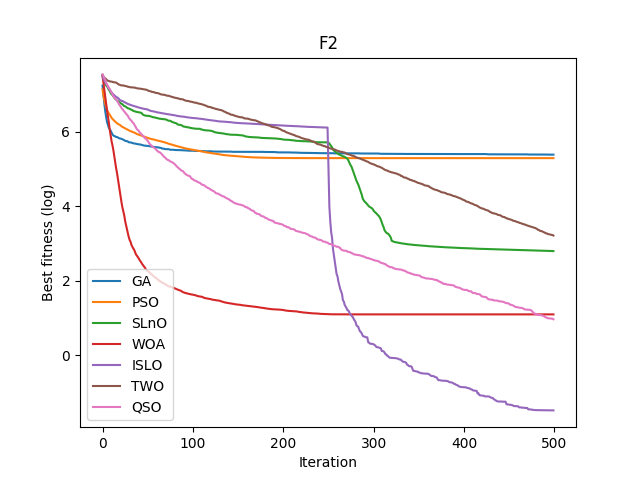
\includegraphics[width=1\linewidth]{png/convergence/islo_uni_F2}
  	 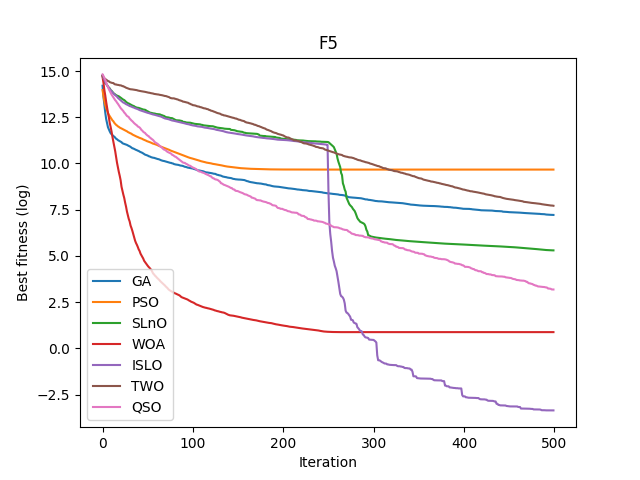
\includegraphics[width=1\linewidth]{png/convergence/islo_uni_F5}
  	 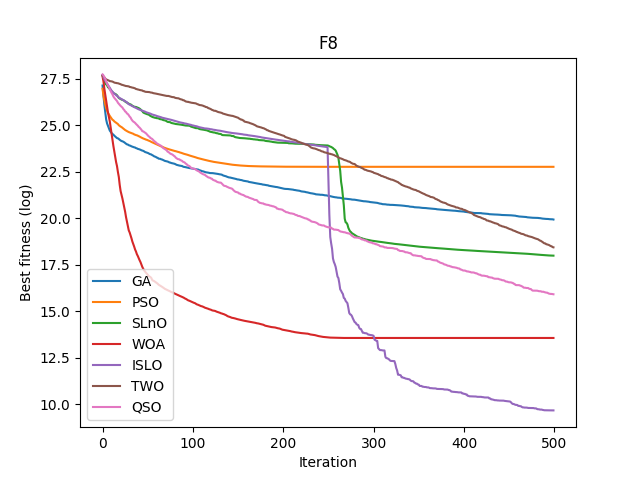
\includegraphics[width=1\linewidth]{png/convergence/islo_uni_F8}
  	\caption{Unimodal}
  	\label{subfig:uni_convergence}
  	\end{subfigure}
   \begin{subfigure}{0.49\textwidth}
   	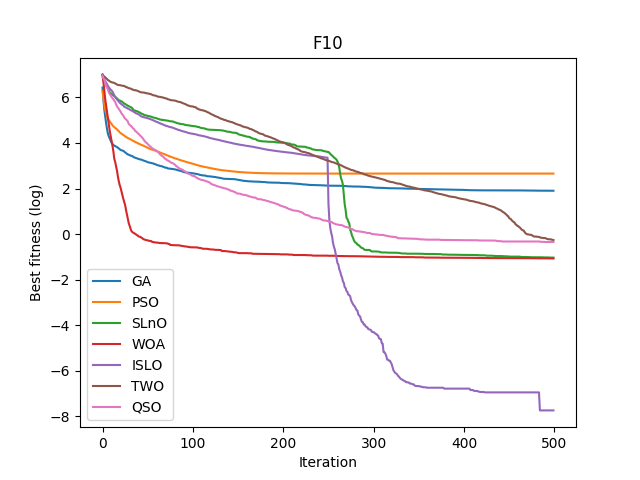
\includegraphics[width=1\linewidth]{png/convergence/islo_multi_F10}
  	 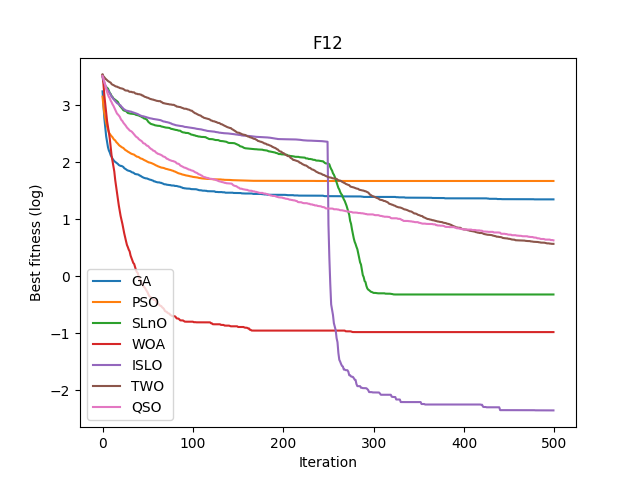
\includegraphics[width=1\linewidth]{png/convergence/islo_multi_F12}
  	 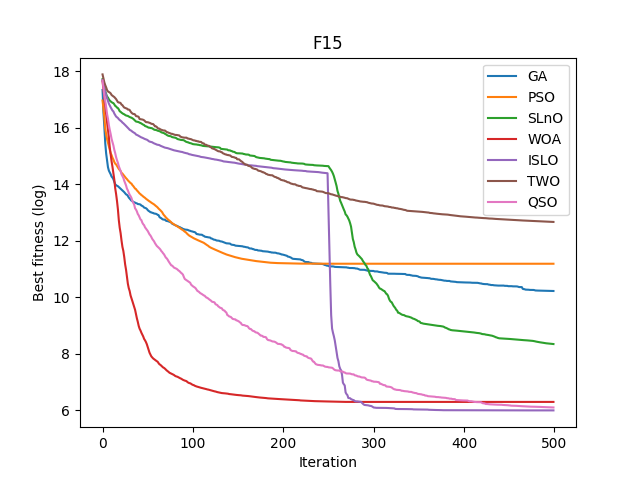
\includegraphics[width=1\linewidth]{png/convergence/islo_multi_F15}
  	 \caption{Multimodal}
  	\label{subfig:multi_convergence}
  	\end{subfigure}
  \caption{Convergence speed of each algorithm on unimodal (a) and multimodal (b) functions.} 
  \label{fig_uni_multi_convergence} 
\end{figure}
	Functions $f_1$ - $f_{16}$ are unimodal and multimodal functions. These kinds of functions are selected following a couple of testing purposes. Specifically, unimodal functions allow us to evaluate exploitation capacity of meta-heuristic optimizers since they only have one global optimal minimum; multimodal functions help us see algorithms' exploration performance with a number of local minimum points, which exponentially increases following the increase in search space dimension. In general, it can be seen from the Table \ref{tbl_results_uni_multi} that ISLO shows the best performance among all chosen algorithms in the most test cases except $f_{11}$. Furthermore, while optimizing several functions, ISLO is able to reach or nearly the optimal value with decent stability.
	 
	\textbf{The accuracy and the stability:} From the gained results of unimodal and multimodal funtions in Table. \ref{tbl_results_uni_multi}, it could be made the following observations:
\begin{itemize}
\item ISLO outperforms the others in all test cases except $f_{11}$. In the experiments with unimodal functions $f_1$-$f_8$, ISLO is the best algorithm in the term of exploitation capacity, being ranked at the first position among all chosen algorithms. The results with functions $f_1$ and $f_3$ indicate that ISLO could lead the population relatively near the global optimal position. Additionally, along with the best results in term of accuracy, ISLO also performs good stability since the standard deviation values are below 1 in all cases, especially in $f_1$ and $f_3$, the $std$ values are mostly 0. The results prove that compared with the original SLnO, ISLO's exploitation ability is significantly enhanced. 
\item The results in Table. \ref{tbl_results_uni_multi} for multimodal functions $f_9$-$f_{16}$ indicate that ISLO also has a superior exploration ability. ISLO stands at the first ranking in 7 out of 8 functions, and with $f_{14}$ and $f_{16}$ ISLO reaches the global optimal values of the functions, accompanying with that is relatively small standard deviation values. It is notable that ISLO is less competitive at $f_{11}$ where it stands at $5th$ position, being outperformed by WOA, TWO and original SLnO. However, in $f_8$, $f_9$, $f_{10}$, $f_{13}$, $f_{14}$ and $f_{16}$, ISLO's results are much better than the others in both terms of accuracy and stability.
\end{itemize}
In summary, all gained results with unimodal and multimodal funtions figure out that ISLO has the excellent exploitation and exploration capacity. This is due to the fact that apart from considering and updating search agents' position following the best agent, taking the best experience of each agent into account (Eq. \ref{islo_eq3}) helps ISLO exploits population's information far better than SLnO. Apart from this, opposition-based updating operation in the exploration phase enrichs the diversity of population, helping ISLO easily jumps out of local minimums.

	\textbf{The convergence speed:} The convergence speed of all algorithms working on several functions are shown in Fig. \ref{fig_uni_multi_convergence}. It is clear that ISLO always considerably enhance its global best fitness values in the second half of the iterations. The reason is that on the first half of th e iterations, ISLO is in its exploration phase (since the value of C during that time is always greater than 1, see Algorithm \ref{algorithm_islo}). After changing to exploitation phase, ISLO has the ability to exploit and converge to global minimum quickly, providing better results than the others. Fig. \ref{fig_uni_multi_convergence} indicates that ISLO is competitive with an acceptable convergence speed, and also providing decent fitness values in functions $f_2$, $f_5$, $f_8$, $f_{10}$, $f_{12} $ and $f_{15}$. SLnO has the same pattern of convergence curves compared with ISLO, but it coverges to mediocre fitness values, especially in $f_2$, $f_5$ and $f_{10}$. Also, WOA and QSO are competitive compared with ISLO in function $f_{15}$, where the final results of them are extremely close to ISLO's.
	
\begin{table}[!t]
\caption{Comparison of optimization results obtained for the hybrid and composition benchmark functions}
\label{tbl_results_hybrid_compos}
\centering
\resizebox{\textwidth}{!}{%
\begin{tabular}{|l|l|l|l|l|l|l|l|l|}
\hline
Function             &      & GA       & PSO      & SLnO     & WOA               & ISLO               & TWO      & QSO               \\ \hline
\multirow{3}{*}{$f_{17}$} & mean & 2.19E+05 & 1.46E+05 & 8.08E+04 & 8.82E+03          & \textbf{1.81E+03}  & 2.08E+06 & 5.46E+03          \\ \cline{2-9} 
                     & std  & 1.29E+05 & 7.68E+04 & 4.92E+04 & 2.63E+03          & \textbf{1.95E+02}  & 7.79E+05 & 5.00E+02          \\ \cline{2-9} 
                     & rank & 6        & 5        & 4        & 3                 & \textbf{1}         & 7        & 2                 \\ \hline
\multirow{3}{*}{$f_{18}$} & mean & 6.43E+06 & 3.15E+04 & 9.29E+05 & 8.12E+03          & 4.46E+03           & 4.73E+05 & \textbf{3.49E+03} \\ \cline{2-9} 
                     & std  & 1.10E+06 & 9.41E+03 & 1.66E+06 & 2.55E+03          & 2.95E+03           & 1.00E+05 & \textbf{8.92E+02} \\ \cline{2-9} 
                     & rank & 7        & 4        & 6        & 3                 & 2                  & 5        & \textbf{1}        \\ \hline
\multirow{3}{*}{$f_{19}$} & mean & 8.97E+03 & 2.36E+03 & 2.48E+03 & 1.95E+03          & \textbf{1.92E+03}  & 9.67E+03 & 2.01E+03          \\ \cline{2-9} 
                     & std  & 2.87E+03 & 9.31E+02 & 8.36E+02 & 4.45E+01          & \textbf{2.08E+00}  & 2.02E+04 & 1.25E+02          \\ \cline{2-9} 
                     & rank & 6        & 4        & 5        & 2                 & \textbf{1}         & 7        & 3                 \\ \hline
\multirow{3}{*}{$f_{20}$} & mean & 1.82E+05 & 2.52E+04 & 1.49E+04 & 2.81E+03          & \textbf{2.12E+03}  & 4.53E+05 & 1.77E+04          \\ \cline{2-9} 
                     & std  & 2.14E+05 & 1.24E+04 & 6.90E+03 & 6.75E+02          & \textbf{8.47E+01}  & 1.03E+06 & 5.70E+04          \\ \cline{2-9} 
                     & rank & 6        & 5        & 3        & 2                 & \textbf{1}         & 7        & 4                 \\ \hline
\multirow{3}{*}{$f_{21}$} & mean & 7.97E+06 & 5.51E+07 & 1.04E+08 & 2.00E+05          & \textbf{3.19E+03}  & 1.79E+08 & 4.43E+08          \\ \cline{2-9} 
                     & std  & 2.95E+06 & 3.76E+07 & 1.00E+08 & 4.37E+05          & \textbf{9.01E+03}  & 8.02E+07 & 1.46E+08          \\ \cline{2-9} 
                     & rank & 3        & 4        & 5        & 2                 & \textbf{1}         & 6        & 7                 \\ \hline
\multirow{3}{*}{$f_{22}$} & mean & 2.28E+05 & 1.26E+07 & 1.85E+08 & 8.72E+02          & \textbf{7.16E+02}  & 1.17E+08 & 2.57E+08          \\ \cline{2-9} 
                     & std  & 7.52E+04 & 1.27E+07 & 6.11E+08 & 2.55E+02          & \textbf{9.38E-01}  & 1.29E+08 & 1.73E+08          \\ \cline{2-9} 
                     & rank & 3        & 4        & 6        & 2                 & \textbf{1}         & 5        & 7                 \\ \hline
\multirow{3}{*}{$f_{23}$} & mean & 5.29E+06 & 6.08E+07 & 2.65E+08 & 3.59E+04          & \textbf{1.26E+03}  & 2.74E+08 & 9.76E+08          \\ \cline{2-9} 
                     & std  & 1.29E+06 & 2.72E+07 & 3.12E+08 & 4.30E+04          & \textbf{1.19E+03}  & 1.57E+08 & 4.46E+08          \\ \cline{2-9} 
                     & rank & 3        & 4        & 5        & 2                 & \textbf{1}         & 6        & 7                 \\ \hline
                     \multirow{3}{*}{$f_{24}$} & mean & 1.12E+04 & 2.96E+04 & 3.46E+03 & 1.92E+03          & \textbf{1.81E+03}  & 1.15E+05 & 2.23E+03          \\ \cline{2-9} 
                     & std  & 2.35E+03 & 1.71E+04 & 1.04E+03 & 4.11E+01          & \textbf{1.62E+00}  & 4.71E+04 & 6.89E+02          \\ \cline{2-9} 
                     & rank & 5        & 6        & 4        & 2                 & \textbf{1}         & 7        & 3                 \\ \hline
\multirow{3}{*}{$f_{25}$} & mean & 8.17E+06 & 1.26E+08 & 8.62E+08 & 1.23E+05          & \textbf{2.95E+03}  & 2.64E+08 & 6.98E+08          \\ \cline{2-9} 
                     & std  & 2.42E+06 & 5.10E+07 & 1.08E+09 & 1.15E+05          & \textbf{4.98E+02}  & 1.09E+08 & 3.18E+08          \\ \cline{2-9} 
                     & rank & 3        & 4        & 7        & 2                 & \textbf{1}         & 5        & 6                 \\ \hline
\multirow{3}{*}{$f_{26}$} & mean & 6.78E+03 & 4.50E+03 & 4.63E+03 & 3.03E+03          & \textbf{2.22E+03}  & 4.20E+03 & 2.82E+03          \\ \cline{2-9} 
                     & std  & 3.59E+02 & 3.76E+02 & 9.84E+02 & 9.60E+02          & \textbf{2.03E+00}  & 2.15E+02 & 3.59E+01          \\ \cline{2-9} 
                     & rank & 7        & 5        & 6        & 3                 & \textbf{1}         & 4        & 2                 \\ \hline
\multirow{3}{*}{$f_{27}$} & mean & 3.22E+03 & 3.15E+03 & 2.52E+03 & 2.43E+03          & \textbf{2.40E+03}  & 2.87E+03 & 2.66E+03          \\ \cline{2-9} 
                     & std  & 6.09E+01 & 1.18E+02 & 1.66E-02 & 3.28E+00          & \textbf{1.50E+00}  & 2.58E+01 & 6.04E+00          \\ \cline{2-9} 
                     & rank & 7        & 6        & 3        & 2                 & \textbf{1}         & 5        & 4                 \\ \hline
\multirow{3}{*}{$f_{28}$} & mean & 2.11E+05 & 5.47E+04 & 1.06E+05 & 9.88E+04          & 8.02E+04           & 1.49E+05 & \textbf{3.25E+03} \\ \cline{2-9} 
                     & std  & 6.99E+03 & 1.22E+04 & 5.84E+03 & 7.98E+03          & 3.86E+04           & 3.89E+03 & \textbf{1.81E+00} \\ \cline{2-9} 
                     & rank & 7        & 2        & 5        & 4                 & 3                  & 6        & \textbf{1}        \\ \hline
\multirow{3}{*}{$f_{29}$} & mean & 3.77E+05 & 1.13E+07 & 2.17E+13 & 2.92E+03          & \textbf{2.83E+03}  & 2.39E+13 & 8.72E+06          \\ \cline{2-9} 
                     & std  & 2.07E+05 & 1.10E+05 & 1.27E+11 & 4.78E+01          & \textbf{5.36E+00}  & 3.05E+11 & 1.90E+06          \\ \cline{2-9} 
                     & rank & 3        & 5        & 6        & 2                 & \textbf{1}         & 7        & 4                 \\ \hline
\multirow{3}{*}{$f_{30}$} & mean & 4.31E+03 & 1.68E+06 & 3.04E+03 & 2.93E+03          & \textbf{2.91E+03}  & 1.12E+04 & 3.21E+03          \\ \cline{2-9} 
                     & std  & 7.28E+02 & 1.94E+06 & 5.60E-01 & 2.30E+00          & \textbf{1.32E+00}  & 1.54E+04 & 1.66E+02          \\ \cline{2-9} 
                     & rank & 5        & 7        & 3        & 2                 & \textbf{1}         & 6        & 4                 \\ \hline
\end{tabular}%
}
\end{table}

\begin{figure}[!ht] 
   \centering
   \begin{subfigure}{0.49\textwidth}
   	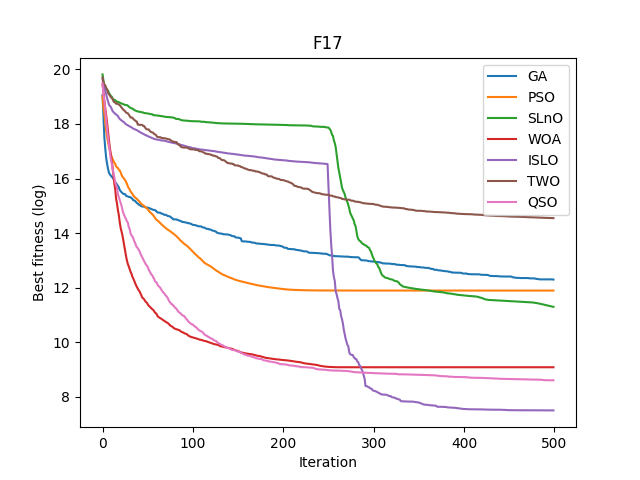
\includegraphics[width=1\linewidth]{png/convergence/islo_hybrid_F17}
  	 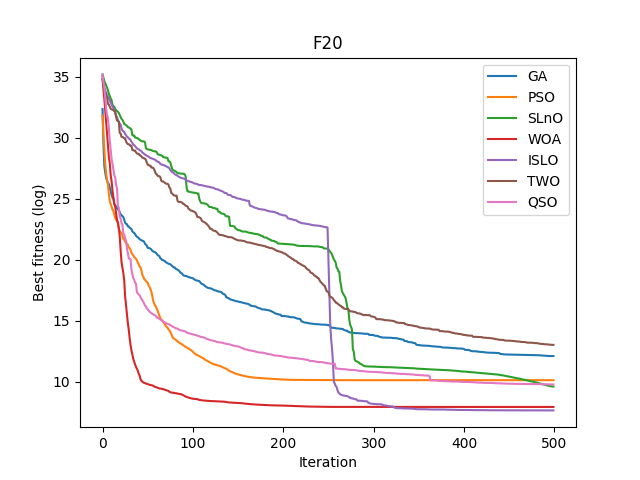
\includegraphics[width=1\linewidth]{png/convergence/islo_hybrid_F20}
  	 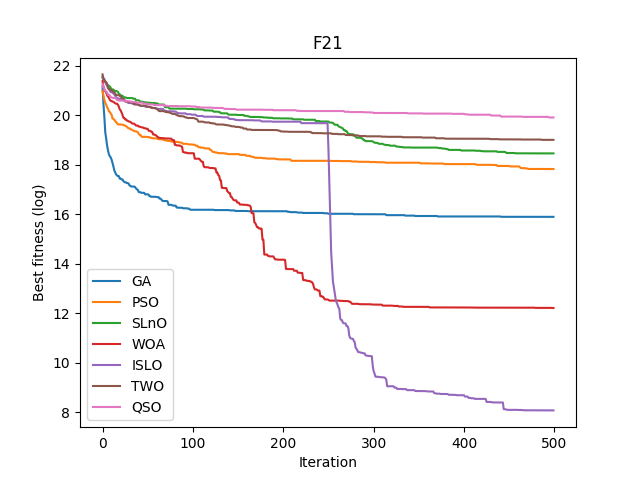
\includegraphics[width=1\linewidth]{png/convergence/islo_hybrid_F21}
  	\caption{Hybrid}
  	\label{subfig:hybrid_convergence}
  	\end{subfigure}
   \begin{subfigure}{0.49\textwidth}
   	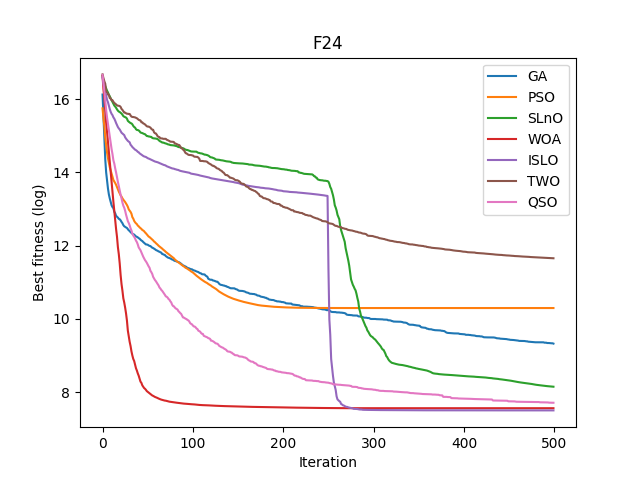
\includegraphics[width=1\linewidth]{png/convergence/islo_compos_F24}
  	 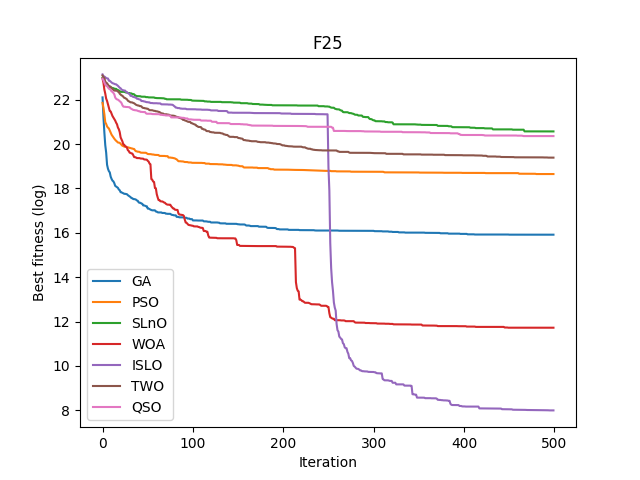
\includegraphics[width=1\linewidth]{png/convergence/islo_compos_F25}
  	 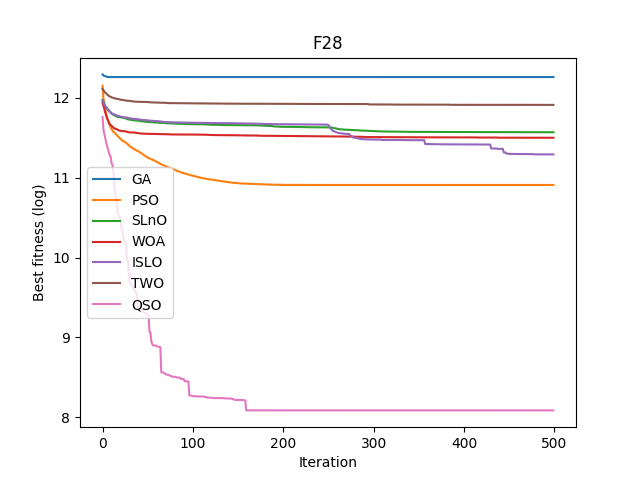
\includegraphics[width=1\linewidth]{png/convergence/islo_compos_F28}
  	 \caption{Composition}
  	\label{subfig:compos_convergence}
  	\end{subfigure}
  \caption{Convergence speed of each algorithm on hybrid (a) and composition (b) functions.} 
  \label{fig_hybrid_compos_convergence} 
\end{figure}
\subsubsection{Hybrid and Composition benchmark functions}

	Functions $f_{17}$-$f_{30}$ are hybrid and composition functions. In hybrid functions ($f_{17}$-$f_{23}$, the variables are randomly divided into subcomponents which play a role as input for different basic functions including both unimodal and multimodal functions. In order to work well on these functions, algorithms are required to be good at both exploitation and exploration capacity, because hybrid functions are both unimodal and multimodal, and they own different properties for different variables subcomponents. On the other hand, optimization of composite mathematical functions ($f_{24}$-$f_{30}$) is a very challenging task, because local optima is only avoided by a proper balance between exploitation and exploration. In general, Fig. \ref{tbl_results_hybrid_compos} shows that ISLO owns the best performance over all hybrid and compostion functions. The results from ISLO stand at first ranking in all cases except $f_8$ and $f_{28}$ where the first position belongs to QSO. Also, as what is observed in Fig. \ref{fig_hybrid_compos_convergence}, ISLO's convergence curves are similar to those in unimodal and multimodal functions, and ISLO still has a very fast convergence after the first half of iteration because of its updating mechanism.
	

	
	\textbf{The accuracy and the stability:} 
	
	To resolve the optimization problem in hybrid functions $f_{17}$-$f_{23}$, it is evident that ISLO can work very well in almost cases. The results shown in Table. \ref{tbl_results_hybrid_compos} indicates that ISLO has the superior results at functions $f_{17}$, $f_{19}$, $f_{20}$ and $f_{23}$ compared with state-of-the-art algorithms such as WOA and QSO. Furthermore, with functions $f_{21}$ and $f_{23}$, ISLO's results are much better than the others', proving good capacity at both exploitation and exploration. Solving the case $f_{18}$, although ISLO does not account for the first place, it is still very competitive when its result is only worse than QSO's.
	
	For composition functions, ISLO shows the best performance among all the algorithms by standing at the first place in 6 out of 7 functions. Specifically, in $f_{24}$, $f_{27}$, $f_{29}$ and $f_{30}$, there is no big differences between ISLO'results and the others', while in $f_{25}$ and $f_{26}$, $mean$ and $std$ values from Table. \ref{tbl_results_hybrid_compos} indicates the dominance of ISLO in optimizing these functions. This proves that ISLO owns a superior balance between its exploitation and exploration while solving test problems. Also $std$ values from ISLO in most cases are below 10, showing the decent stability of this algorithm compared with GA or PSO algorithms.
	
	\textbf{The convergence speed:} As working on unimodal and multimodal functions, when working on hybrid and composite mathematical functions, ISLO still owns the fast convergence in the second half of iterations. The convergence curves in Fig. \ref{fig_hybrid_compos_convergence} shows that ISLO starts to converge very fast right after exploration phase comes to an end. In $f_{17}$ and $f_{24}$, the convergence curves indicate that ISLO is very competitive with WOA because these 2 algorithm converge to almost one value. Also, the results comes from ISLO is far better than the original SLnO in all cases, proving that exploitation and exploration capacities in SLnO are considerably enhanced. QSO is observed to be superior in function $f_{28}$, in which the others including ISLO are stuck in local minimums.   

\section{Application}
\label{sec:exp_app}
	
	In this section, proposed model in Section \ref{sec:application} is utilized for solving time-series prediction in the auto-scaling problem in cloud computing. Our experiment is done with 4 datasets: Google Trace CPU, Google Trace Memory, EU Internet Traffic and UK Internet Traffic. In this empirical study, ISLO-CFNN model is compared with several deep learning models such as simple MLP, the original CFNN, and two well-known and widely used models in time-series forecasting: LSTM and GRU in terms of accuracy, run time and the number of hyper-parameters. Also, optimizing capacity of ISLO on CFNN is compared with several swarm-based algorithms in Section \ref{sec:exp_theory}. The bio-inspired models used to validate against ISLO-CFNN are PSO-CFNN and SLnO-CFNN, which are CFNN models optimized by PSO and SLnO algorithms, respectively.
	
	We would first describe 4 datasets used in this experiment. Then, the parameter setting for each model and evaluation metrics are introduced in detail. Finally, ISLO-CFNN performance is compared with the deep learning models as well as bio-inspired models in different perspectives.

\subsection{Dataset and Set up}
\label{exp:data}

\subsubsection{Google Trace dataset}
	The most important dataset in our experiments is gathered by Google on a cluster of about $12500$ machines \cite{reiss2011google} during 29 days, starting from May 2011. Resources requirement and usage data for each jobs are recorded by each machine in cluster, and then the data is managed by cluster's management system. In Google Trace dataset, there are two columns, which are about two extremely important information of Central Processing Unit (CPU) and Random Access Memory (RAM) required for each job. For that reason, we decide to choose these two information as two time-series datasets (called Google Trace CPU and Google Trace RAM from here). The datasets are processed and summarized in 5-minute interval, containing 8351 data points, and considered as the total demand for resources in the whole Google's cluster. Visualization of Google Trace CPU and Google Trace RAM datasets is illustrated in Fig. \ref{fig_data_ggtrace}. 
	
\begin{figure}[!ht] 
   \centering
   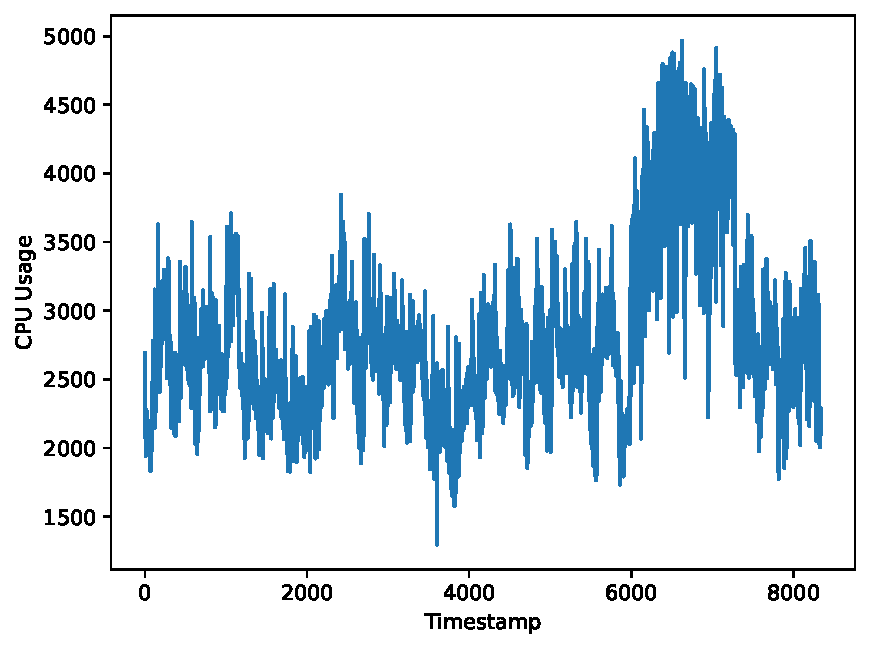
\includegraphics[width=0.49\linewidth]{/pdf/dataset/cpu_full}
   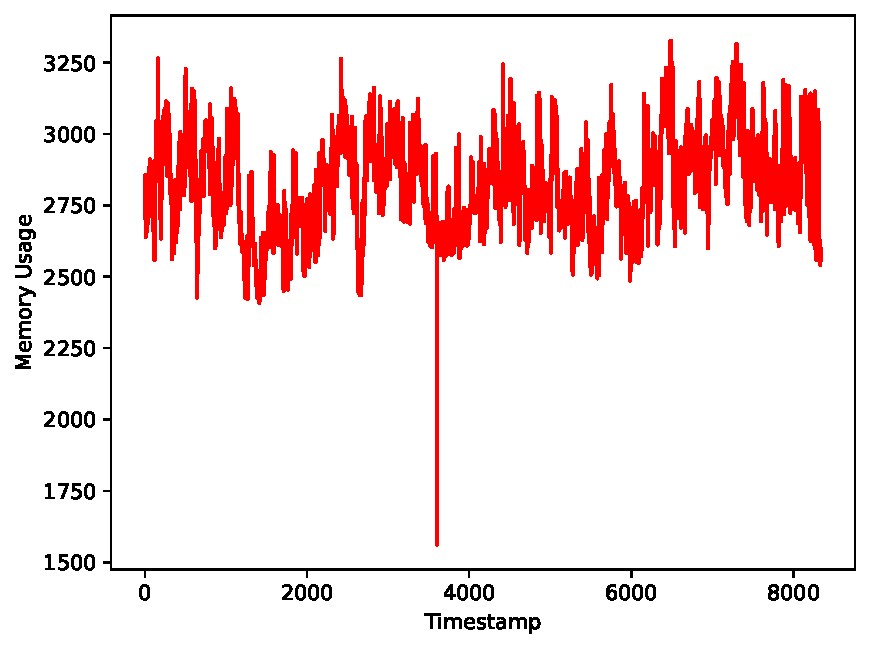
\includegraphics[width=0.49\linewidth]{/pdf/dataset/ram_full}
  \caption{Visualization of Google Trace CPU (left) and Google Trace RAM (right) datasets.} 
  \label{fig_data_ggtrace} 
\end{figure}
	
\subsection{Collecting data}
\label{collect_data}
 
\subsubsection{EU Internet Traffic and UK Internet Traffic datasets}
	
	These two sets of data, which is used for experiments in \cite{cortez2012multi}, are recorded by two distinct ISPs. The EU Internet Traffic dataset comes from a private ISP playing a role as a reporter with centers  in 11 European cities. The data corresponds to a a transatlantic link and was collected from 06:57 hours on 7 June to 11:17 hours on 29 July 2005. The UK Internet Traffic is derived from m UKERNA and represents aggregated traffic in the United Kingdom academic network backbone. It was
reported between 19 November 2004, at 09:30
hours and 27 January 2005, at 11:11 hours. Both of two datasets are processed and summarized in every 5 minutes, creating EU Internet Traffic (14773 records) and UK Internet Traffic (19989 records) as the input in our experiments. 2D visualization of the data is shown in Fig. \ref{fig_data_it} as below.

\begin{figure}[!ht] 
   \centering
   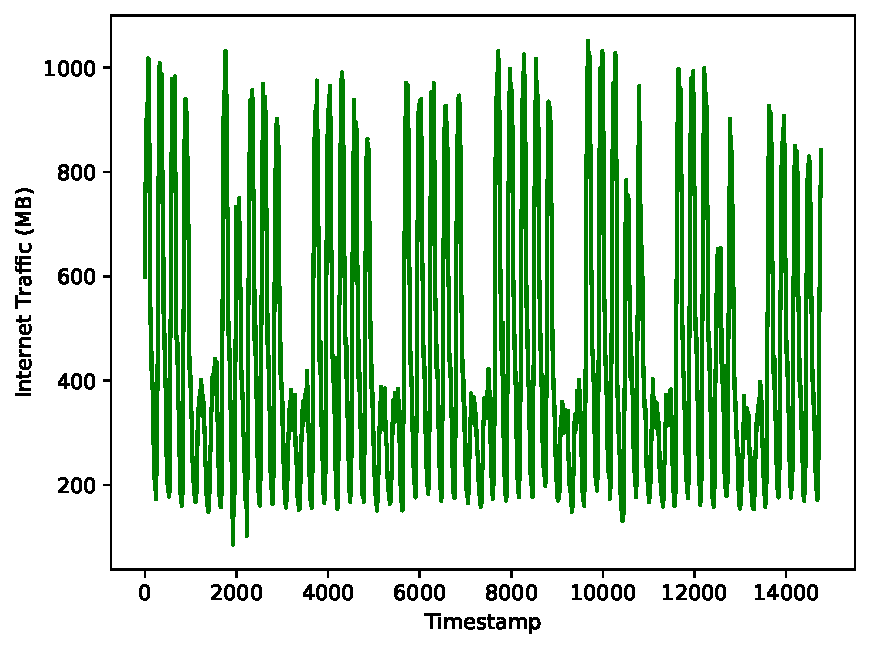
\includegraphics[width=0.49\linewidth]{/pdf/dataset/it_eu}
   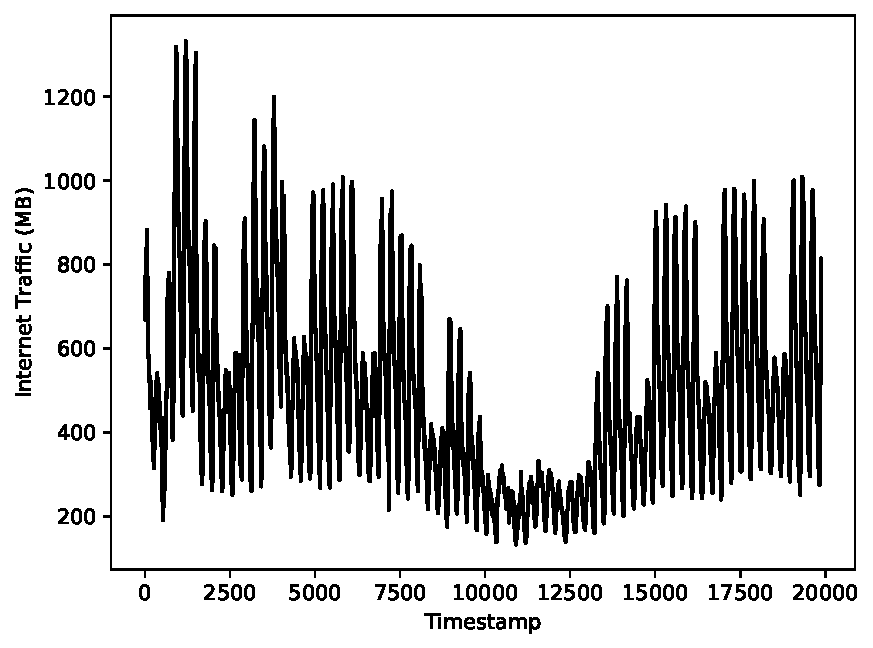
\includegraphics[width=0.49\linewidth]{/pdf/dataset/it_uk}
  \caption{Visualization of EU Internet Traffic (left) and UK Internet Traffic (right) datasets.} 
  \label{fig_data_it} 
\end{figure}

  

\subsection{Parameter Setting and Evaluation Metrics}
	
	As mentioned above, ISLO-CFNN's performance is compared with 4 deep learning models: MLPs, CFNN, LSTM and GRU, and 2 bio-inspired models: PSO-CFNN and SLnO-CFNN models. The hyper-parameter settings for each model are described as below:
\begin{itemize}
\item 4 datasets used for these experiments are all divided into 2 sets: training set and testing set with the ratio 0.8:0.2. The training set accounts for the first 80\% of the datasets, and the remaining is of testing set because of the sequential characteristic of time-series data.
\item CFNN's architectures in all models are configured with the same structure with three layers: input layer, one hidden layer and output layer which contains only one neuron in time-series prediction.
\item The input size for all models is 3 as we use 3 historical data points to predict the output in current time (mentioned in Section \ref{sec:application}).
\item RNN-based models as LSTM and GRU contains one input layer, LSTM (or GRU) blocks and one output layer with the same hyper-parameter setting as described in \cite{fu2016using}.
\item In all test, including with deep learning models and swarm-based algorithms, the number of iterations is set to 1000. From the experiments, we figure out that the amount of 1000 iterations is enough for all algorithms to converge to their final results. 
\end{itemize} 

Besides the common settings for models, the following settings are applied for each swarm-based algorithms as they show the best empirical performance:

\begin{itemize}
\item The population size for each algorithm is set to 200.
\item For PSO, based on the original paper \cite{eberhart1995particle}, cognitive learning rates $c_1=c_2=2.05$, and inertia factor $w$ is set linearly reducing from 0.9 to 0.4 over the course of iterations.
\item For SLnO and ISLO, hyper-parameters are set as described in original paper \cite{masadeh2019sea}, and also, $c_1$ and $c_2$ in ISLO algorithm are the same as shown for PSO.
\end{itemize}

\subsection{Results and Discussion}  
	


\chapter{Conclusions}

\appendix
% appendices come here

\bibliographystyle{plain}
\bibliography{references}
%\addcontentsline{toc}{chapter}{Bibliography}
%\bibliographystyle{alpha}
%\bibliography{bibliography/bibliography}

\end{document}